\documentclass[../notes.tex]{subfiles}

\pagestyle{main}
\renewcommand{\chaptermark}[1]{\markboth{\chaptername\ \thechapter\ (#1)}{}}
\setcounter{chapter}{4}

\begin{document}




\chapter{Sequencing and Organelles}
\section{Sequencing and Next-Generation Sequencing}
\begin{itemize}
    \item \marginnote{10/25:}Yamuna wants us to call her by her first name.
    \item Spends the first 5 minutes glowing about teaching the class.
    \item As a postdoc, Yamuna worked at the bench next to the guys who developed Illumina sequencing.
    \item Sequencing represents the best of biochemistry because you have to know the chemistry to do it and the biology to interpret the results.
    \item Doing science via discovery (e.g., why is the sky blue?) vs. understanding (e.g., how does this work?).
    \begin{itemize}
        \item Chemical biology is the science of invention because you are trying to take the natural and control it.
    \end{itemize}
    \item What Yamuna wants us to take away: Understand how polymerases and everything works and then be able to tell what our sequence is.
    \begin{itemize}
        \item Sequencing is an exercise in tweaking the chemistry of biomolecules to get a certain result, enabled by the fact that we understand it so well.
    \end{itemize}
    \item DNA sequencing: Maxam-Gilbert, Sanger, Pyro (454) sequencing, Illumina, Nanopore, SMRT.
    \item Two principles that underlie DNA sequencing.
    \begin{itemize}
        \item Size-based separation on a gel (esp. for the older ones).
        \item \textbf{PCR}.
    \end{itemize}
    \item \textbf{Polymerase chain reaction}: A technique that amplifies (rapidly duplicates) a certain sequence of DNA millions or billions of times. \emph{Also known as} \textbf{PCR}.
    \begin{itemize}
        \item Suppose you have a strand of DNA and you want to know the sequence of a 150 bp bit.
        \item You need sufficient and sufficiently pure starting material to begin. Thus, if we have 50-100 copies of the DNA from extraction and mince them, the pieces will come out in different lengths.
        \item But we need way, way more copies to do meaningful chemistry and, moreover, we need only copies of the one specific set of base pairs.
        \item Solution: Polymerase chain reaction uses RNA polymerase, dNTPs, \ce{Mg^2+}, and some other things to make many many copies of just the 150 bps you're interested in.
        \item You need a primer (about 20-30 base pairs; what is necessary for specificity) that will sit on the beginning of the region.
        \item PCR uses a thermal cycler (a fancy oven that heats and cools between temperatures of your choosing at a rate of your choosing).
        \item DNA in an Eppendorf tube in the thermal cycler. We heat it to unwind the strands and then break the hydrogen bonding, yielding single-stranded DNA. Our forward and reverse primers sit on the single strands at the beginning of our target region. DNA polymerase attaches and copies until it falls off. Then we repeat.
        \item With every cycle, we increase/amplify the number of copies of target DNA vs. the variable length DNA. Thus, the variable length becomes more of an impurity. Now we can start to do chemistry.
        \item PCR was invented by Kary Mullis (who Yamuna isn't a fan of because he was a heavy user of LSD, downplayed humans' role in climate change, and doubted that HIV is the sole cause of AIDS).
        \item How do you create the primer if you haven't sequenced the DNA yet??
    \end{itemize}
    \item Separating DNA duplexes on the basis of size/length (\emph{not} polarity) using Agel (which is fancy TLC).
    \begin{itemize}
        \item If DNA is small, it will easily snake through the gel. If it is big, it will take longer.
        \item Like gel electrophoresis, you still have a cathode and anode. DNA (negatively charged due to phosphate groups) will move toward the cathode.
        \item Entirely pure substrate $\to$ one band.
        \item You can separate 48 bp strands from 49 bp strands.
        \item You have to chop up your DNA into reasonable sizes so that it can separate on a gel: 1000 vs. 1001? Not possible. 100 vs. 99? Possible. Resolution is better.
    \end{itemize}
    \item Huntington's genetic test.
    \begin{itemize}
        \item There is a protein/gene called Huntington. Everyone has a short number of repeats on the Huntington protein, but if you have two many (40+), you will develop Huntington's disease.
        \begin{itemize}
            \item 26-27 repeats is the border. This issue arises from polymerase "going nuts" and adding more repeats than it meant to.
            \item A \textbf{pathogenic} number of repeats vs. you being fine.
        \end{itemize}
        \item Amplify the section of your DNA containing the repeats. Then it is not necessary to sequence and count; you just need to determine the length of the repeating strand.
    \end{itemize}
    \item Cystic fibrosis.
    \begin{itemize}
        \item Often results from the $\Delta F508$ mutation (single AA mutation at phenylalanine 508).
        \item Yamuna's cousin died aged 36 from cystic fibrosis, but it wasn't $\Delta F508$ --- it was two "variant of unknown significance" mutations. Cases like hers allow us to canonize the noncanonical mutations.
    \end{itemize}
    \item 10 years, \$1 billion to sequence the entire human genome using Sanger sequencing (slow and very expensive).
    \begin{itemize}
        \item Someone else envisioned sequencing the entire human genome for \$1000 in a day.
        \item If feasible, it would have been great to understand all genomes, but instead, it helped us with COVID (detecting variants in a population and a person, virility, capacity for transmission).
        \item This saved many people by prevention (e.g., travel restrictions) before a cure (like the "mRNA vaccines") existed.
    \end{itemize}
    \item Back in 2005 when Yamuna started her lab in India, she would get data as a \textbf{sequence chromatogram}.
    \item \textbf{Seqeunce chromatogram}: A graph consisting of various colored peaks, each corresponding to one type of base pair.
    \begin{figure}[h!]
        \centering
        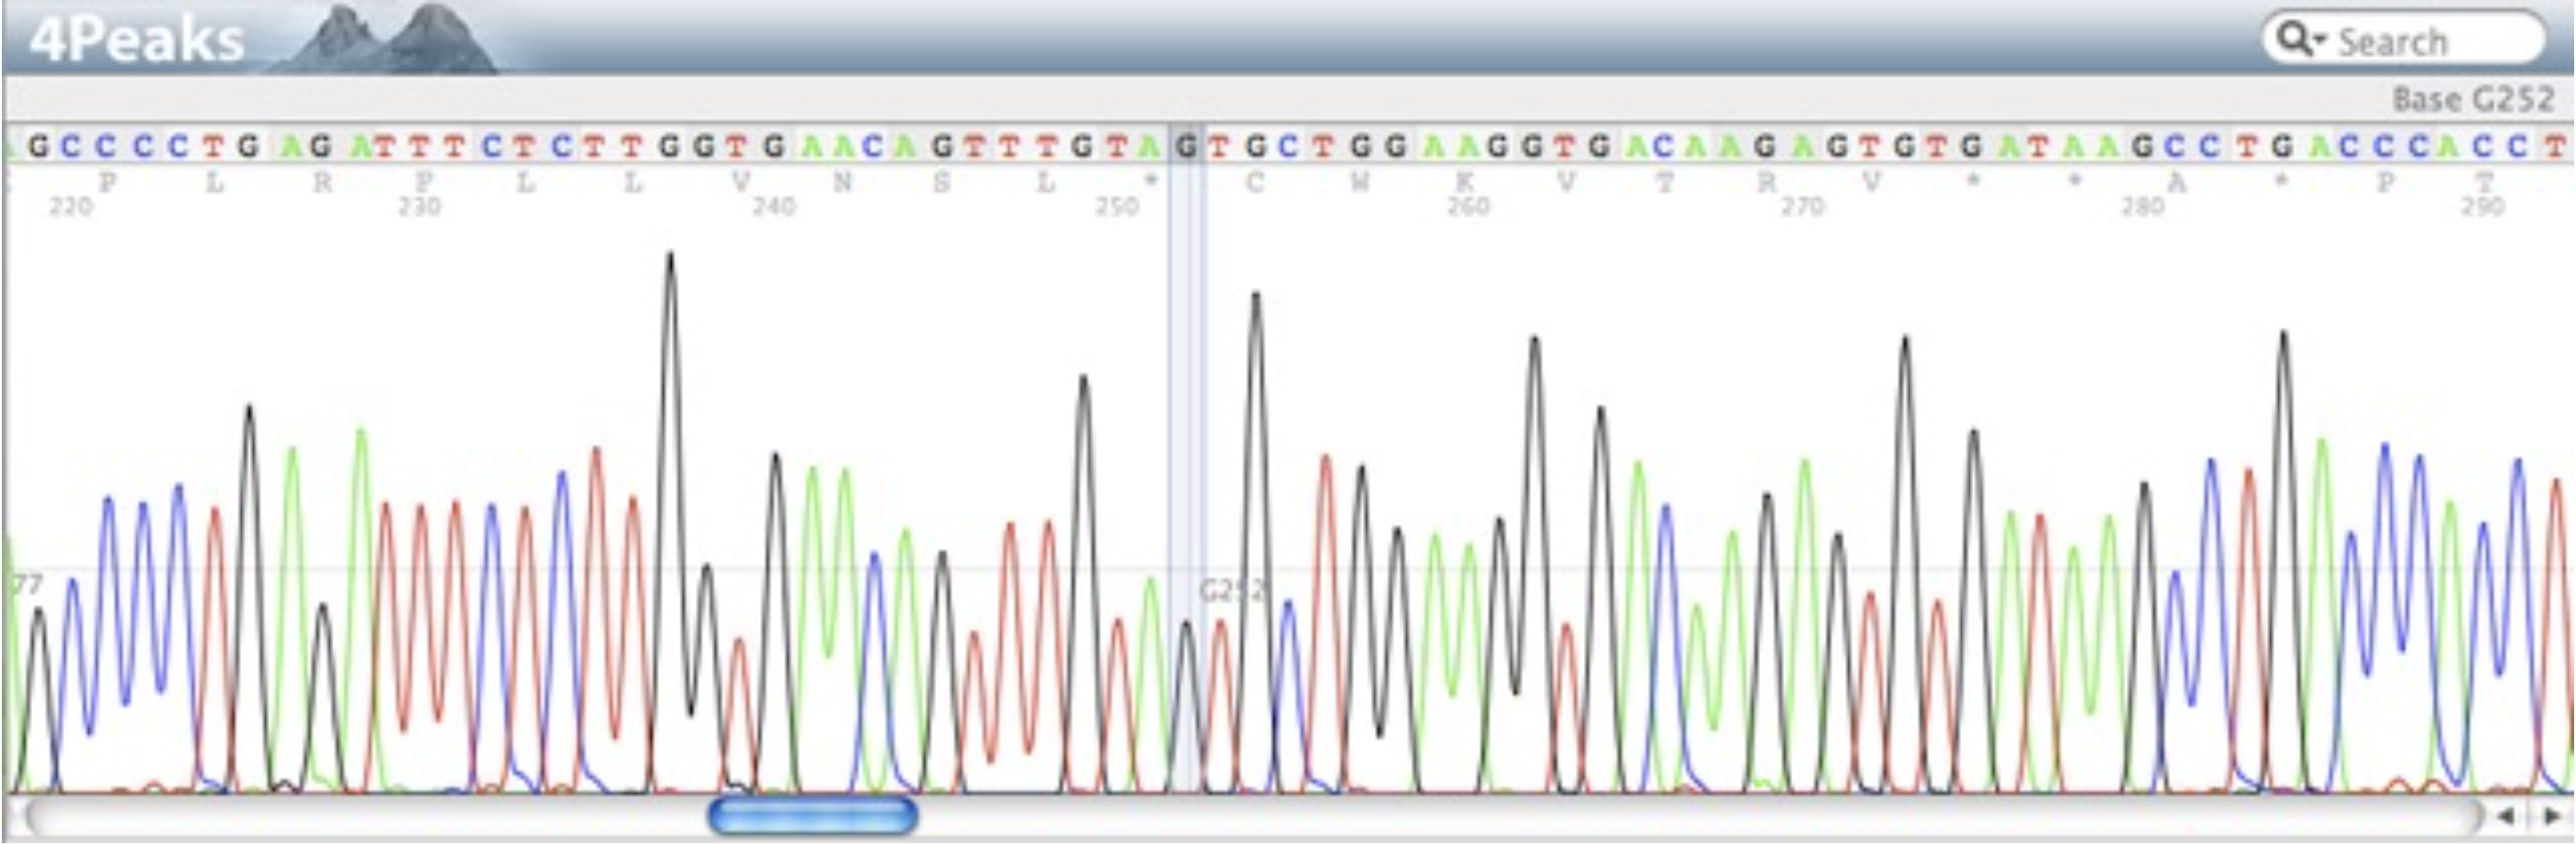
\includegraphics[width=0.7\linewidth]{../ExtFiles/sequenceChromatogram.png}
        \caption{Sequence chromatogram example.}
        \label{fig:sequenceChromatogram}
    \end{figure}
    \begin{itemize}
        \item Blue peak: Cytosine, Green peak: Adenine, Red peak: Thymine, Black peak: Guanine.
        \item Idiot-proofed for biologists to just read off their sequence from the top of the display window.
        \item How the graph is generated (briefly; this is Sanger sequencing).
        \begin{itemize}
            \item You write the sequence based on the length of the strand and how far it travels and which fluorescent dye has been attached to our gene.
            \item When DNA is being built, different dNTPs come in and sample the active site. If hydrogen bonding is correct, DNA polymerase locks into place, fuses it to the $3'$ end of the growing strand, and releases a \textbf{pyrophosphate}.
            \item This only happens when you have the right dNTP (there are energy barriers if you have the wrong one based on faulty hydrogen bonding).
            \item Release of a pyrophosphate is key to another sequencing method.
            \item Ability to make DNA artificially in a chemistry lab (Caruthers, 1985). You can attach literally anything to the growing $3'$ end. This allows you to create primers that set an address.
            \begin{itemize}
                \item Yamuna believes this should have won a Nobel prize since it's been the basis for several others.
            \end{itemize}
            \item If you attach a ddNTP to the growing end, you stop growth.
        \end{itemize}
    \end{itemize}
    \item \textbf{Pyrophosphate}: Two phosphates bound via a single linking oxygen, i.e., \ce{P2O7^4-}. \emph{Denoted by} \textbf{PPi}.
    \item Maxam-Gilbert sequencing.
    \begin{itemize}
        \item Developed by Wally Gilbert and Allan Maxam.
        \begin{itemize}
            \item Gilbert and Sanger originally won the Nobel Prize for sequencing.
        \end{itemize}
        \item Know this for historical reasons; came out second, but was adopted first.
        \item Start with a bunch of copies (circa 1 million) of a DNA strand obtained using bacterial cloning.
        \item Label the $5'$ end of each sequence with \ce{{}^32P}.
        \item Divvy up the labeled DNA between four Eppendorfs. To each tube, add a chemical that is selective for one or two nucleobases. Add just enough of the chemical so that every strand will react once. Remember that most strands will not react. Then introduce hot piperidine (Yamuna said hydrazine??) to cleave the strand right before (Yamuna says after??) the modification.
        \item Chemicals:
        \begin{align*}
            \text{A}+\text{g} &= \ce{HCOOH}&
            \text{G} &= \ce{Me2SO4}&
            \text{T}+\text{c} &= \ce{N2H4}&
            \text{C} &= \ce{N2H4 + NaCl}
        \end{align*}
        \item Running these mixtures on a gel will lead to bands corresponding to each cut and unreacted strands.
        \item The strand that travels the farthest (is the lightest/shortest) corresponds to the first nucleobase. The strands that travel the least are the unreacted strands.
        \begin{itemize}
            \item Example 1: No band in the $\text{T}+\text{c}$ column and a band in the $\text{C}$ columns? Cytosine.
            \item Example 2: Bands at the same level in the $\text{A}+\text{g}$ and $\text{G}$ columns? Guanine.
        \end{itemize}
    \end{itemize}
    \item Sanger sequencing.
    \begin{itemize}
        \item When cloning became pass\'{e}, everyone switched to Sanger.
        \item Two methods of Sanger sequencing: Sequential and parallel.
        \item Sequential Sanger sequencing.
        \begin{itemize}
            \item Amplify your region of interest using PCR.
            \item However, during this process, add a small amount (1-5\%) of a specific dideoxynucleotide (ddNTP). If you include a small amount of ddATP for example, then whenever DNA polymerase matches one of these with a thymine and incorporates it into the growing strand, the strand will not be able to grow any further (there is no longer a $3'$ hydroxyl to bond the next nucleotide to).
            \item This will allow you to generate stops at every nucleobase of a certain type.
            \item Doing this for every nucleobase independently and then running all four samples on a gel gives you a similar result to Maxam-Gilbert sequencing, except that this time, our result is analogous to cleaving after the "modification" and we don't have "leaks" as with the $\text{T}+\text{c}$ and $\text{A}+\text{g}$ chemicals.
        \end{itemize}
        \item Parallel Sanger sequencing.
        \begin{itemize}
            \item Amplify your region of interest using PCR.
            \item However, during this process, add a small amount (1-5\%) of fluorophore-labeled ddNTPs such that each of the four ddNTPs fluoresces a different color. Incorporating these will guarantee that each strand of DNA ends in a fluorophore-labeled ddNTP.
            \item These strands can be separated with high accuracy using capillary gel electrophoresis.
            \begin{itemize}
                \item Capillary gel electrophoresis is very fancy gel --- very long and very thin.
            \end{itemize}
            \item As each strand moves through the capillary, it eventually passes by a light fluorescence detector.
            \item This generates the sequence chromatogram.
        \end{itemize}
        \item Better since it doesn't have radioactivity, once fluorophores became stable, and after the advent of capillary gel electrophoresis.
    \end{itemize}
    \item Svante P\"{a}\"{a}bo at the Max Planck Institute won the 2022 Nobel Prize in Physiology or Medicine for sequencing the Neanderthal genome.
    \begin{itemize}
        \item He extracted DNA from skulls and bones. Every bit of DNA was missing something, but by sequencing enough and comparing, he was able to fully reconstruct it.
        \item He did this with \textbf{pyrosequencing}, which many biologists had forgotten about.
    \end{itemize}
    \item \textbf{Pyrosequencing}: A sequencing by synthesis method that works as follows. \emph{Also known as} \textbf{454 sequencing}. \emph{Procedure}
    \begin{enumerate}
        \item Begin with a pure set of DNA sequences generated via PCR. Bind adapters to the sequences, and biotin to the adapters. Immobilize multiple copies of each sequence on a number of streptavidin beads.
        \item Bind a primer to each sequence and attach DNA polymerase.
        \item Add a specific dNTP (dATP, dTTP, dGTP, or dCTP).
        \item Suppose the first base to be sequenced/synthesized is adenine and dATP is the first dNTP added. Then DNA polymerase will click dATP into place, releasing a pyrophosphate.
        \item The PPi is used by ATP-sulfurylase to generate a molecule of ATP.
        \item This allows Luciferase to use ATP and its substrate to generate a flash of light.
        \item Before adding in another type of dNTP, it is necessary to remove the previous one. This is accomplished by adding apyrase, an enzyme that converts all available dNTPs to dNDPs and then inactive dNMPs.
        \item Counting the number of flashes of light after a dNTP is produced tells us how many of that dNTP in a row there are at that point.
    \end{enumerate}
    \item Example of pyrosequencing.
    \begin{itemize}
        \item Consider the strand ATGGCCC.
        \item Introducing dATP, dGTP, or dCTP at first will lead to no flashes of light. Introducing dTTP will lead to one flash of light (because T binds with A and there is one A).
        \item Similarly, introducing anything other than dATP next will lead to nothing, and introducing dATP will lead to one flash of light.
        \item Now introducing dCTP will lead to two consecutive flashes of light (as two pyrophosphates are released from the addition of two dCTPs to the growing strand, one for each dGTP in the guiding strand).
        \item Lastly, introducing dGTP will lead to three consecutive flashes of light. 
    \end{itemize}
    \item Notes on pyrosequencing.
    \begin{itemize}
        \item 454 is what the company referred to the technology as before it was released and named "pyrosequencing."
        \item Pyrosequencing is the bridge between the ways Yamuna used as a grad student and what we do today.
        \item In an analogy, ATP-sulfurylase is like the light switch, luciferase is like the lightbulb, and apyrase is like the eraser between steps.
        \item You generate a bead with many copies of a specific strand on it.
        \item How this works in a system:
        \item Take DNA, sonicate it to break it up, make the library, add adapters.
        \item Amplify using emulsion PCR (little droplets of water in a mix of oil that contain dNTPs, primers, water, polymerase, etc.).
        \item Relation to chemistry 1-bead, 1-compound question.
        \item During emulsion PCR, the strand that is not covalently bonded (i.e., the newly synthesized one) comes back and reattaches.
        \item PCR amplification occurs until every strand displays the same DNA sequencing.
        \item Many wells; each one contains a single DNA sequence. Then flow in dATP plus an enzyme cocktail.
        \item You need a big flash of light (multiple photons --- 20-30 flashing at the same time).
        \item Your computer flows in different bases to different wells and looks for what gives you a flash.
        \item Allows you to sequence in a massively parallel way.
    \end{itemize}
    \item Illumina sequencing (currently the most important method).
    \begin{itemize}
        \item Sequences 200-300 bps at a time.
        \item Nanopore and SMRT sequencing give you extremely long sequences, but most big biological discoveries today are based on Illumina sequencing.
        \item Once you have your sequences of interest, you attach primers and...
        \item Attach your strands to the surface of a wafer.
        \item Bridge synthesis on the wafer.
        \item You get a flash of light whenever you add.
        \item You get an answer from your entire surface instead of just a single molecule. Since DNA polymerase makes errors, this eliminates them via the law of averages.
        \item The cost of sequencing is now in storing the data, not in the reagents.
        \item Five major challenges to solve to achieve next generation sequencing (NGS) by Illumina.
        \begin{itemize}
            \item The $3'$ OH problem.
            \begin{itemize}
                \item If you want to protect the $3'$ OH with a fluorophore, you have a 2 hour deprotonation. This means that it will take 25 days to sequence 300 bases.
                \item If you use 2-o-nitrophenol, you have a UV-deprotonation. Instaneous but skin cancer.
                \item Single color readout is impractical; thus, you need a four-color readout.
                \item The ideal $3'$ OH protecting group is small, stable under aqueous conditions, has quantitative cleavage and high turnover, and preserves the DNA integrity.
            \end{itemize}
            \item The fluorophore problem.
            \item The polymerase problem.
            \item The surface chemistry problem.
            \item The problem of polymerase-generated errors and parallelization.
        \end{itemize}
    \end{itemize}
    \item Check out videos online.
\end{itemize}



\section{Cell Biology for Chemists}
\begin{itemize}
    \item \marginnote{10/27:}Yamuna starts by telling us that we should feel free to sleep through class and watch the recording if we want since it's so early.
    \item Today: Third-generation sequencing (left over from last class) and then the cell.
    \item So far: Biomolecules, structure, and function. Third generation sequencing will show you how we can assemble all of these components together to get them to do very complex work in union in a very purified way.
    \begin{itemize}
        \item After that, we will focus on how they all function together in the cell.
    \end{itemize}
    \item Yamuna used to think that the cytoplasm was mostly water with a few stray biomolecules, but in reality, there are tons of biomolecules all crammed together into a highly viscous "hot pot" that these components have to navigate through.
    \begin{itemize}
        \item Another factor is quick recognition and selectivity; since biomolecules bump into so many things so quickly, they have to be able to tell what they \emph{don't} want to interact with very quickly after collision.
    \end{itemize}
    \item Illumina qualifies as second-generation sequencing.
    \begin{itemize}
        \item It is still limited to 200-300 base pairs at a time. You can't do an entire run at once. Thus, if you want to sequence repeat regions (such as at the end of telomeres), you can't tell how many repeats you have using such methods.
        \begin{itemize}
            \item This repeat problems is one of the reasons they declared the Human Genome Project concluded but "90\% finished."
            \item After solving the repeats issue, then they declared that the work was done.
            \item Another reason was that they wanted to make their data public so Craig Venter didn't copyright it and freeze science.
        \end{itemize}
    \end{itemize}
    \item \textbf{SMRT sequencing}: A method of sequencing in which DNA polymerase is immobilized over a camera that records each fluorophore flash as nucleotides are added. \emph{Also known as} \textbf{single-molecule real-time sequencing}, \textbf{PacBio sequencing}.
    \begin{figure}[h!]
        \centering
        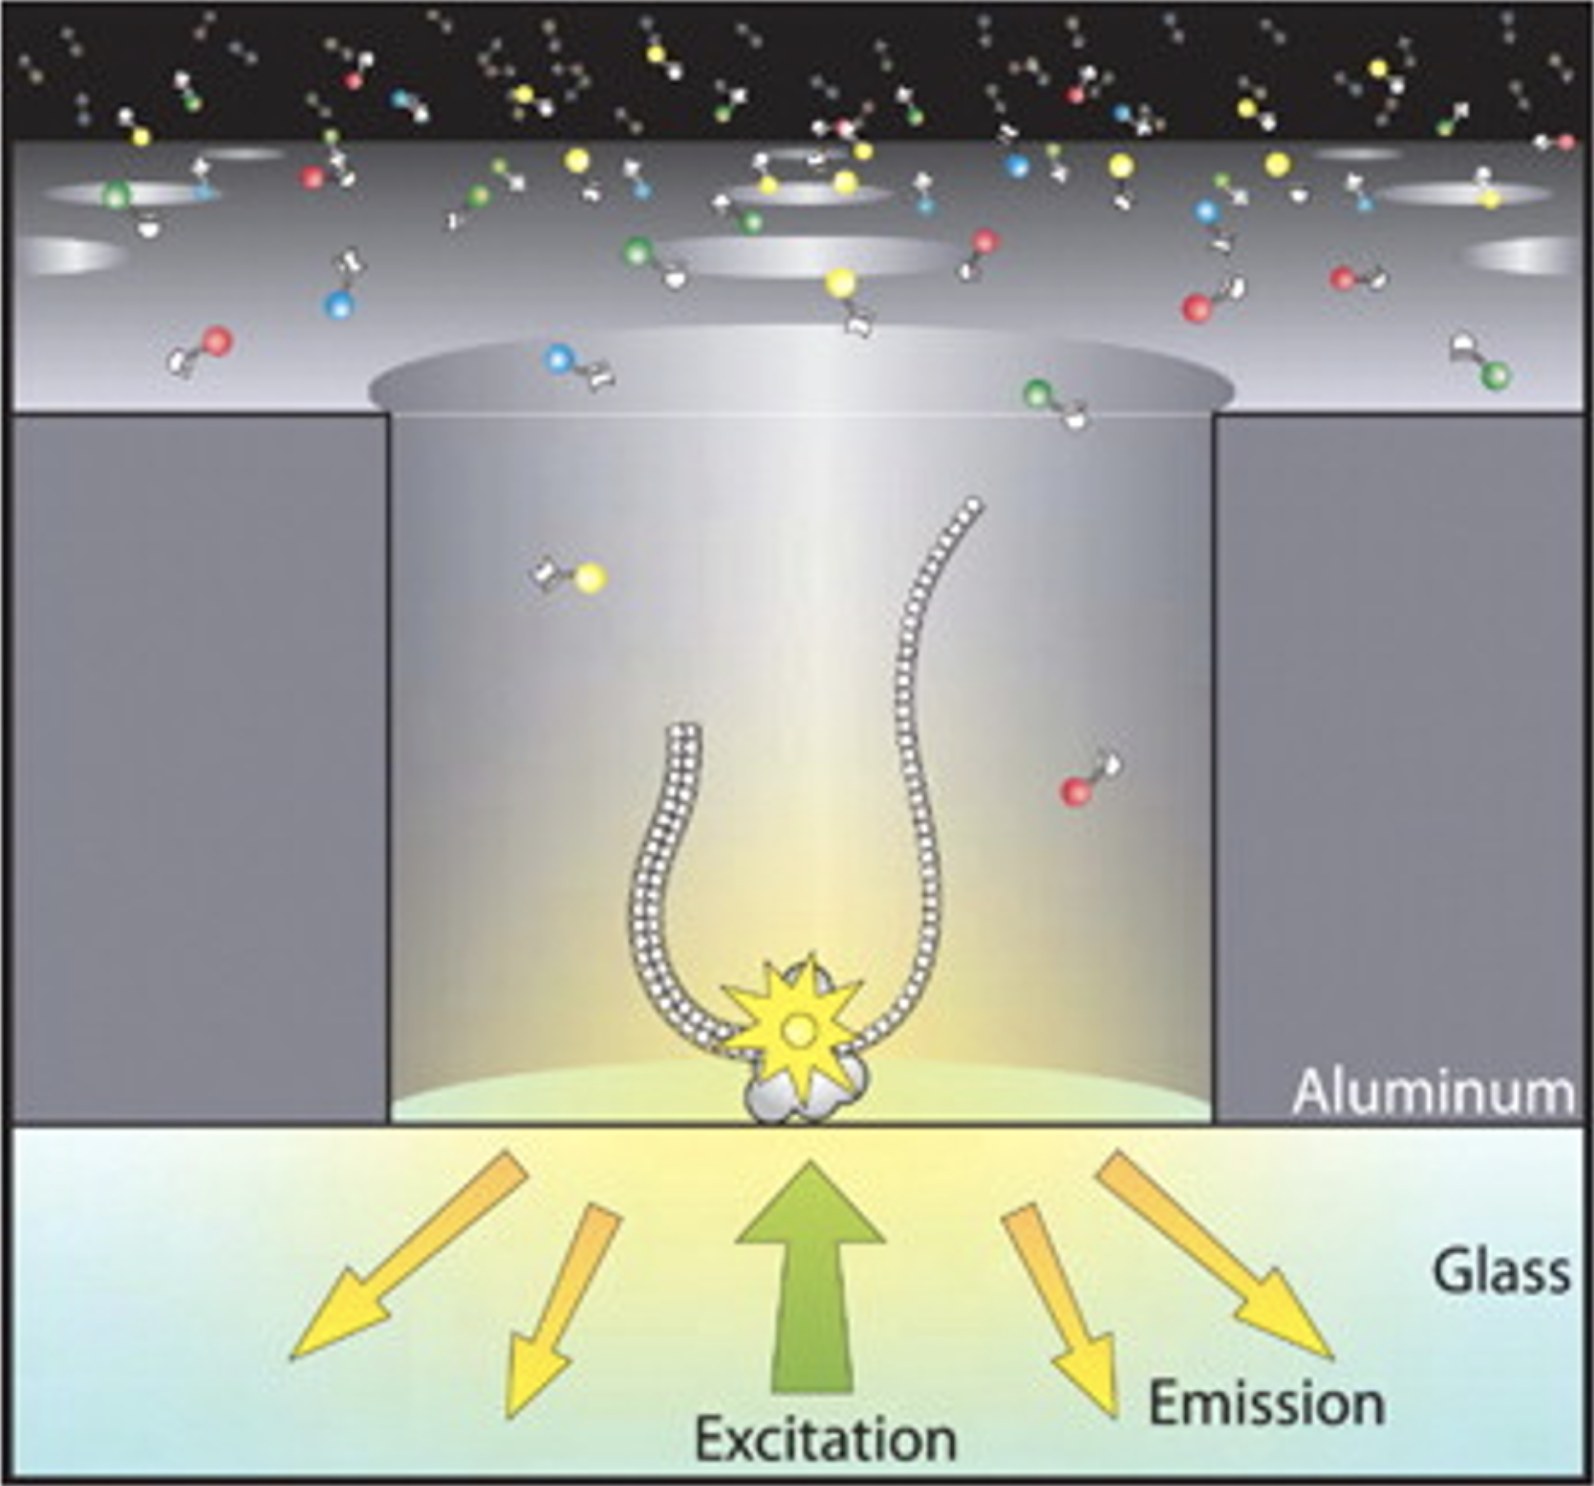
\includegraphics[width=0.4\linewidth]{../ExtFiles/sequencingSMRT.png}
        \caption{SMRT sequencing setup.}
        \label{fig:sequencingSMRT}
    \end{figure}
    \begin{itemize}
        \item A type of third-generation sequencing.
        \item Called real-time because a DNA polymerase is immobilized on a surface; dNTPs carrying fluorophores float in the mix; and as each dNTP is added to the strand by the DNA polymerase, you observe it fluorescing red, green, yellow, or blue exactly when it is added. A camera counts the sequence of colors.
        \item But how do you selectively get the fluorescence of just the base that is added? You fix the DNA polymerase above a \textbf{zero-mode waveguide}.
    \end{itemize}
    \item \textbf{Zero-mode waveguide}: An ultrasmall pore, smaller than the wavelength of light, over which a biomolecule can be held. \emph{Also known as} \textbf{ZMW}.
    \begin{itemize}
        \item In our example, DNA polymerase is held over the pore.
        \item The gap is so small that light passing through it can only interact with the DNA polymerase fixed directly above it and cannot travel further up into the rest of the matrix.
        \item In effect, a ZMW is a "short-sighted fluorescence microscope."
    \end{itemize}
    \item More on the ZMW.
    \begin{itemize}
        \item One of the smallest possible detection volumes.
        \item Developed by Watt W. Webb.
        \item Because the light that comes in has very small wavelength, it cannot travel upwards. You have the greatest intensity right where the light comes in, and then the intensity really falls off; thus, other dNTPs cannot be irradiated.
        \item Notice that all fluorophores are attached at the $3'$ (??) $\gamma$ phosphate, so when a dNTP is added, the pyrophosphate plus fluorophore is sliced out, resulting in a flash of light.
        \item The process occurs in parallel in thousands (now millions) of ZMWs per SMRT cell.
    \end{itemize}
    \item Difference from illumina sequencing: Illumina is not real time.
    \begin{itemize}
        \item DNA polymerase goes so fast naturally (too fast for any camera) that you have to slow it down.
        \item You slow it down by attaching a protecting group to all dNTP's $3'$ phosphates. This group must be removed by a deprotection before the next base can be added.
    \end{itemize}
    \item \textbf{Nanopore sequencing}: An electrical sequencing method currently in development.
    \begin{figure}[h!]
        \centering
        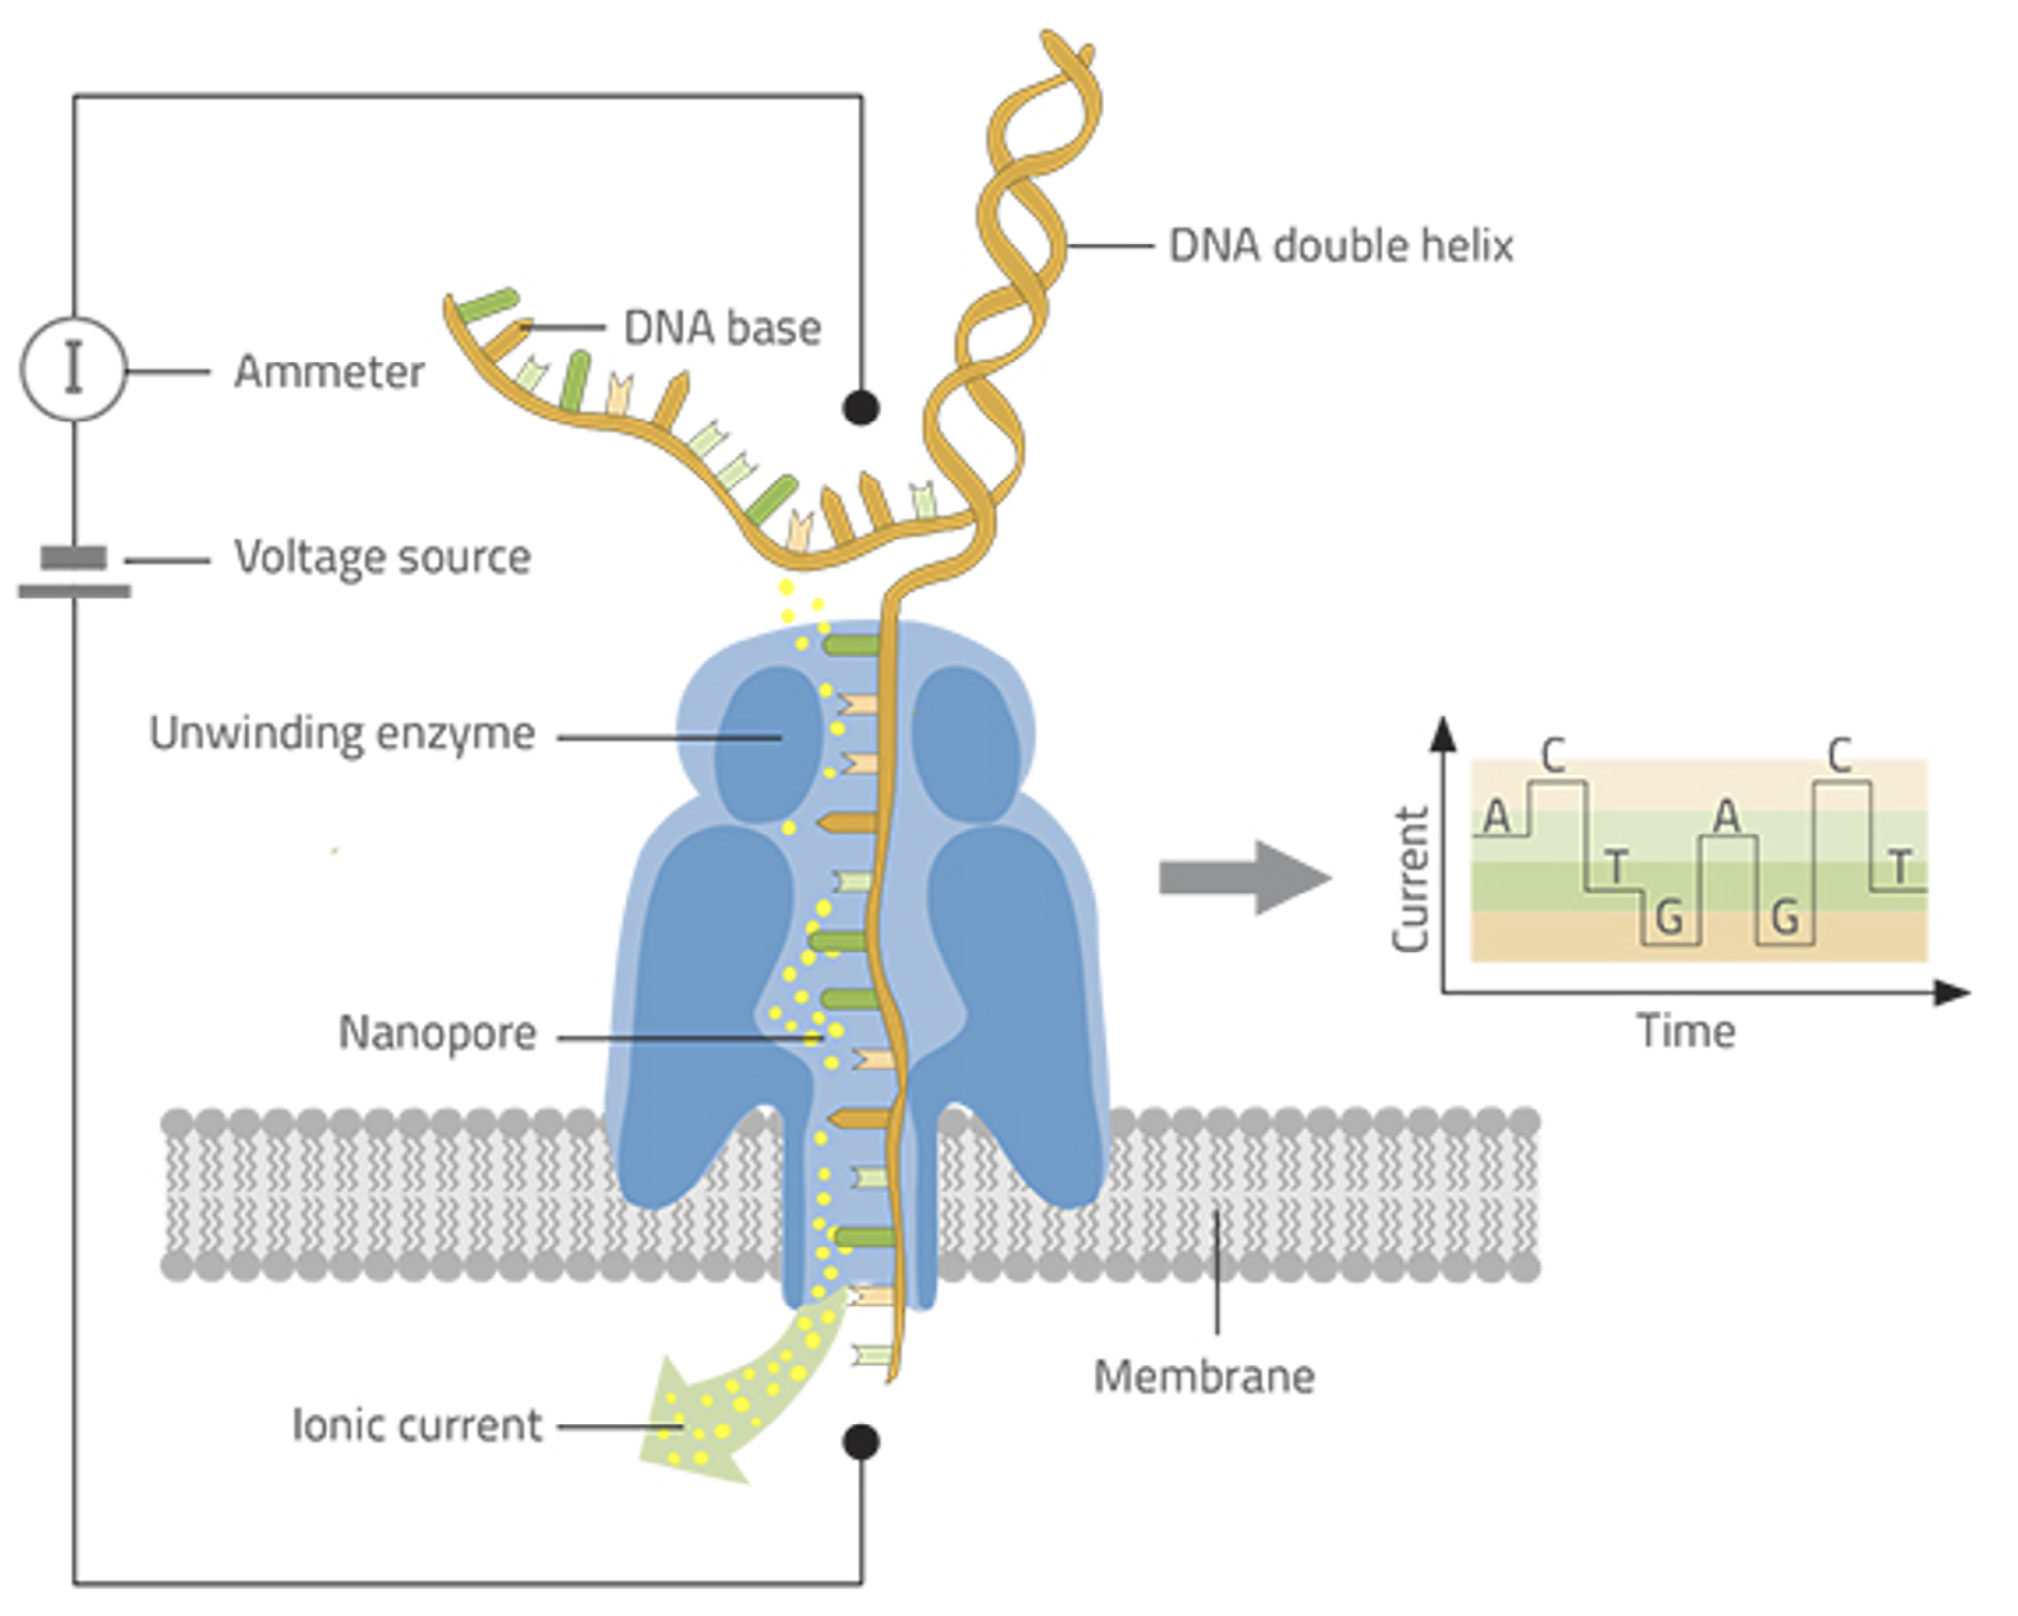
\includegraphics[width=0.4\linewidth]{../ExtFiles/sequencingNanopore.png}
        \caption{Nanopore sequencing setup.}
        \label{fig:sequencingNanopore}
    \end{figure}
    \begin{itemize}
        \item A company has proposed that sequencing can be done on-site using a device the size of a USB drive.
        \item This method of sequencing is electrical, not chemical like all of the others.
        \item The pore (a \textbf{porin}) is of bacterial origin.
        \item Helicase sits at the top, unwinding incident DNA so that one single strand fits through the pore and the other doesn't.
        \item Each base passing through the pore blocks it to a different and unique extent, changing the ion flow through the pore, facilitating sequencing by current.
        \item This method also facilitates sequencing of modified nucleobases (e.g., methylated cytosine or adenine) because they will provide a unique current, too.
    \end{itemize}
    \item Note on the quiz.
    \begin{itemize}
        \item We will need to learn about \textbf{ChIP-Seq}.
    \end{itemize}
    \item \textbf{ChIP-Seq}: A technique that identifies which proteins sit where on the genome. \emph{Also known as} \textbf{chromatin immunoprecipitation and sequencing}.
    \begin{itemize}
        \item Enables us to, for example, find out where in the genome a particular transcription factor sits.
        \item ChIP-Seq accomplishes this by \textbf{immunoprecipitating} the transcription factor.
        \item Immunoprecipitation \textbf{cross-links} the transcription factor to the DNA.
        \item You sonicate the DNA to break it into different bits and then pull down specifically your protein and DNA sequence. Thus, all instances of your protein come down along with all DNA to which it was bound at the time of cross-linking.
        \item Lastly, you sequence the immunoprecipitated DNA and compare it to reference DNA to locate it within the genome.
    \end{itemize}
    \item \textbf{Immunoprecipitation}: Making a biomolecule more heavy so that it can be precipitated out of solution by attaching an antibody to it.
    \begin{itemize}
        \item Achieved by introducing a targeted antibody into the system.
    \end{itemize}
    \item \textbf{Cross-linking} (DNA): The process of covalently binding cellular proteins to DNA.
    \begin{itemize}
        \item This typically occurs upon exposure to various \textbf{endogenous}, environmental, and chemotherapeutic agents.
    \end{itemize}
    \item \textbf{Endogenous} (biomolecule): A biomolecule that grows or originates from within an organism.
    \item A good book to study this content is \emph{Molecular Biology of the Cell} by Bruce Alberts.
    \item Aside: Yamuna's perspective on pharma and biotech companies --- there are three kinds of people in chemical biology.
    \begin{enumerate}
        \item \textbf{Assassins} are asked to develop a molecule that selectively binds a specific family of biomolecules, and they use all of the tools of chemistry and biology to do so.
        \item \textbf{Recruiters} are asked to find the best way to inhibit a certain type of protein.
        \item \textbf{Deciders} decide what pathway should be targeted.
    \end{enumerate}
    \item Deciders are fairly small in number and consult for a variety of companies because they have the vision to know what to do.
    \item We now conclude sequencing and move onto studying the cell.
    \item What makes a city alive?
    \begin{itemize}
        \item Class-suggested answers: Memory, people, energy, and interaction networks.
        \item We should see a cell the way we see a city.
    \end{itemize}
    \item Aspects of a city.
    \begin{itemize}
        \item Transportation, currency flow, executive function, import and export, infrastructure, schools, energy, defense systems, cleaners, the postal system, hospitals, and people/parts.
    \end{itemize}
    \item Analogies within a cell.
    \begin{itemize}
        \item Postal system: Golgi.
        \item Energy: Mitochondria.
        \item Garbage disposal: Lysosomes.
        \item Defense systems and repair: DNA repair mechanisms.
        \item Border: Cell membrane.
        \item Transport system: Microtubules and the cytoskeleton.
        \begin{itemize}
            \item Allow you to go from the membrane to deep within the cell.
            \item Proteins don't migrate by random diffusion but catch hold of an actin network and move.
        \end{itemize}
        \item Factories: Ribosomes are protein production factories.
    \end{itemize}
    \item MicroRNAs largely regulate various networks and exist for robustness.
    \item The cell is alive because all of these parts have to interact with each other. All of their functions are highly interlinked.
    \item Look up the difference between plant and animal cells! Will be an exam question!!
    \begin{itemize}
        \item Plant cells have \textbf{plasmodesmata}, a \textbf{cell wall}, a \textbf{central vacuole}, and \textbf{chloroplasts}.
        \item Animal cells have \textbf{centrioles}.
    \end{itemize}
    \item The plasma membrane: Basics.
    \begin{itemize}
        \item The fluid mosaic model. We are taught in school that the plasma membrane is a homogeneous sea of lipids that proteins are mixed into. However, this is \emph{very} wrong.
        \item The plasma membrane is the first line of defense for the cell against invading pathogens.
        \item This region is really important.
        \begin{itemize}
            \item The first-most drugged class of molecules is \textbf{G-protein coupled receptors}.
            \item The second-most drugged class of molecules is cell-surface ion channels.
        \end{itemize}
        \item A phospholipid has a hydrophilic head and a hydrophobic tail.
        \begin{itemize}
            \item We may approximate them as cylinders according to ??.
            \item The hydrophilic heads face outwards, and the hydrophobic tails face inwards.
        \end{itemize}
    \end{itemize}
    \item \textbf{G-protein coupled receptor}: A protein that is present on the cell surface. \emph{Also known as} \textbf{GPCR}.
    \item The plasma membrane: Main constituents.
    \begin{figure}[h!]
        \centering
        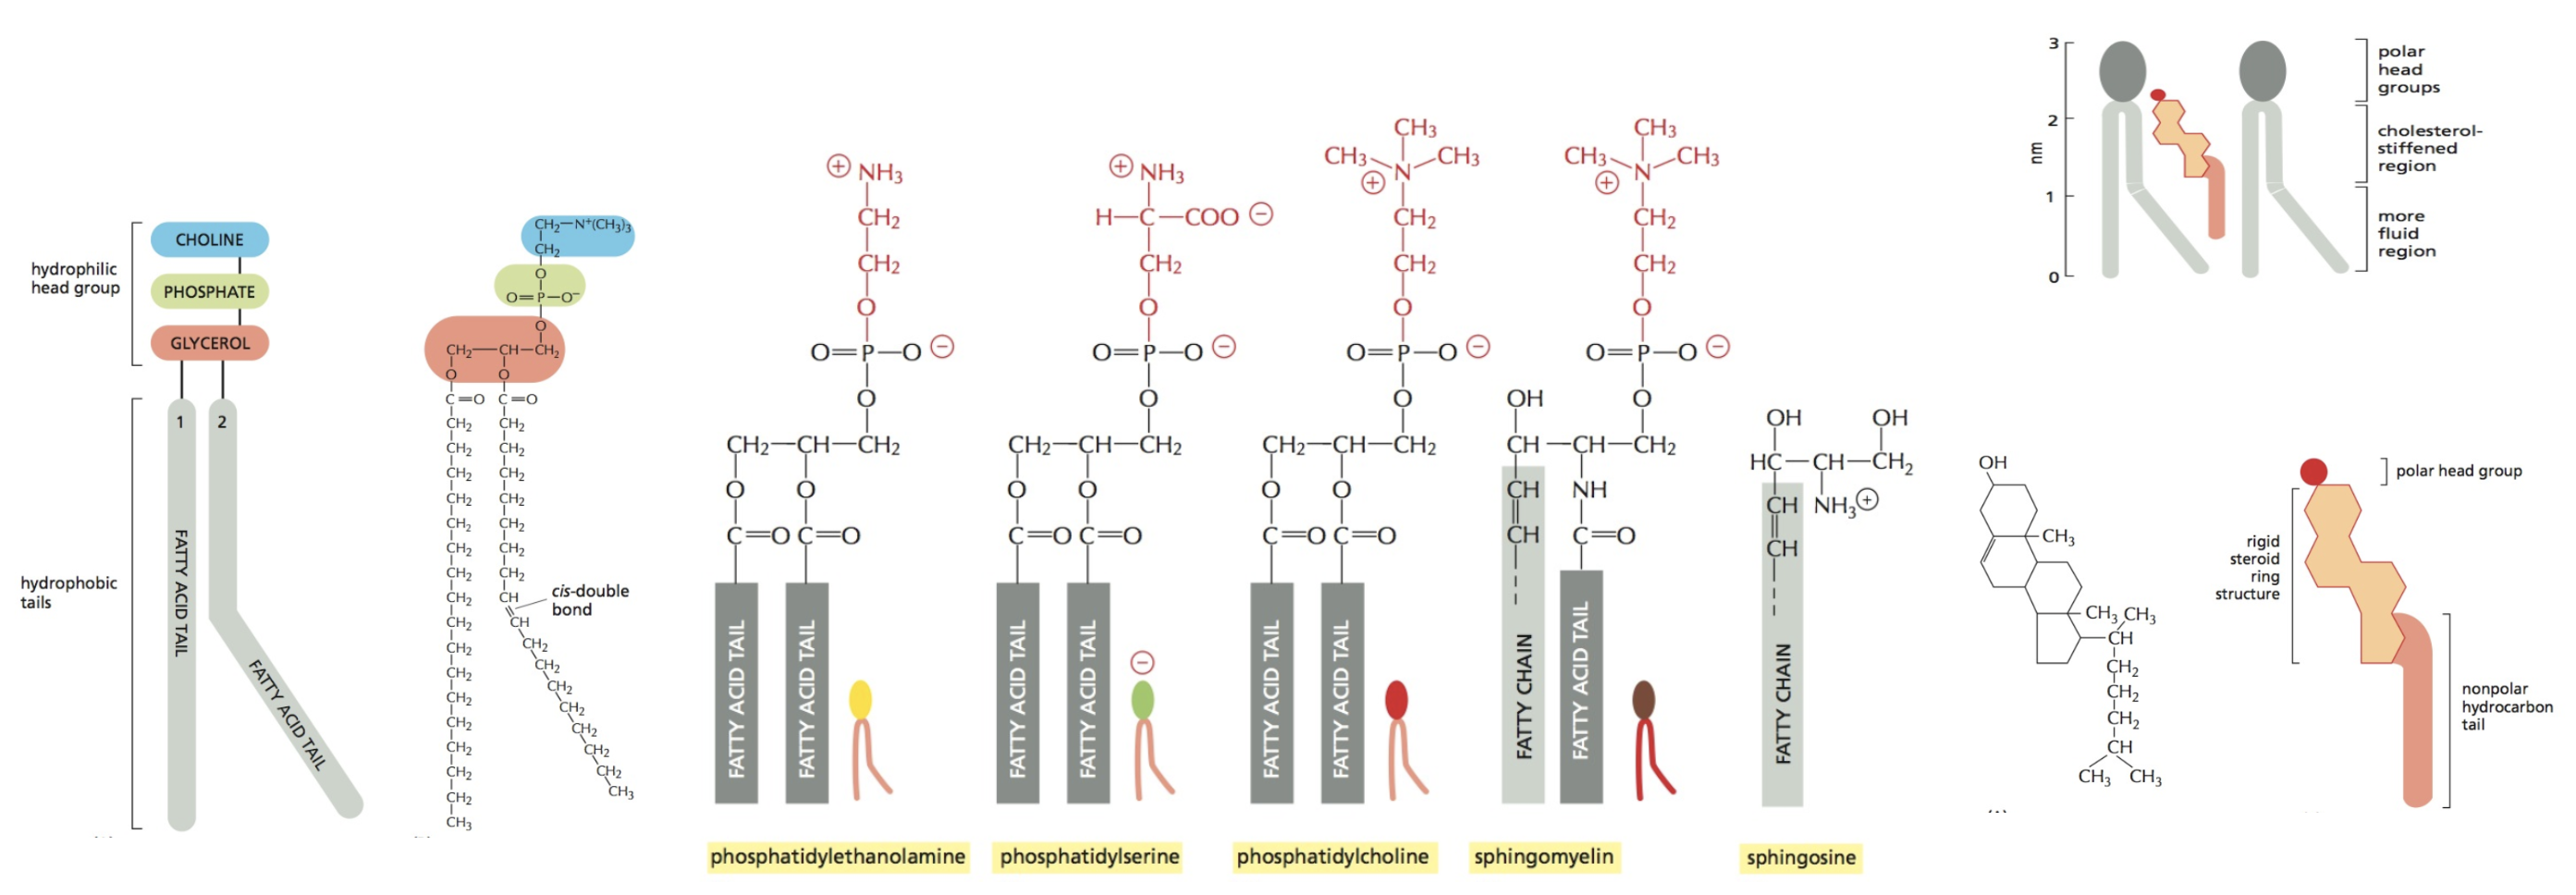
\includegraphics[width=0.98\linewidth]{../ExtFiles/plasmaMembraneConstituents.png}
        \caption{Plasma membrane constituents.}
        \label{fig:plasmaMembraneConstituents}
    \end{figure}
    \begin{itemize}
        \item Comprised of 500-2000 different kinds of lipids molecules; it is not homogeneous.
        \item The variations come from different alkyl chain lengths and degrees of unsaturation. You can also have different head groups: The most common are phosphatidylethanolamine, phosphatidylserine (PS), phosphatidylcholine, and sphingomyelin.
        \item You also have 17-23\% cholesterol in the membrane to provide thermal stability; more than that makes the membrane too stiff, less than that makes the membrane too wobbly.
        \item Cholesterol sits in the membrane wherever the unsaturations are. Unsaturations cause bends which allow cholesterol to slide in and stabilize the system.
    \end{itemize}
    \item The plasma membrane is asymmetric.
    \begin{figure}[H]
        \centering
        \begin{subfigure}[b]{\linewidth}
            \centering
            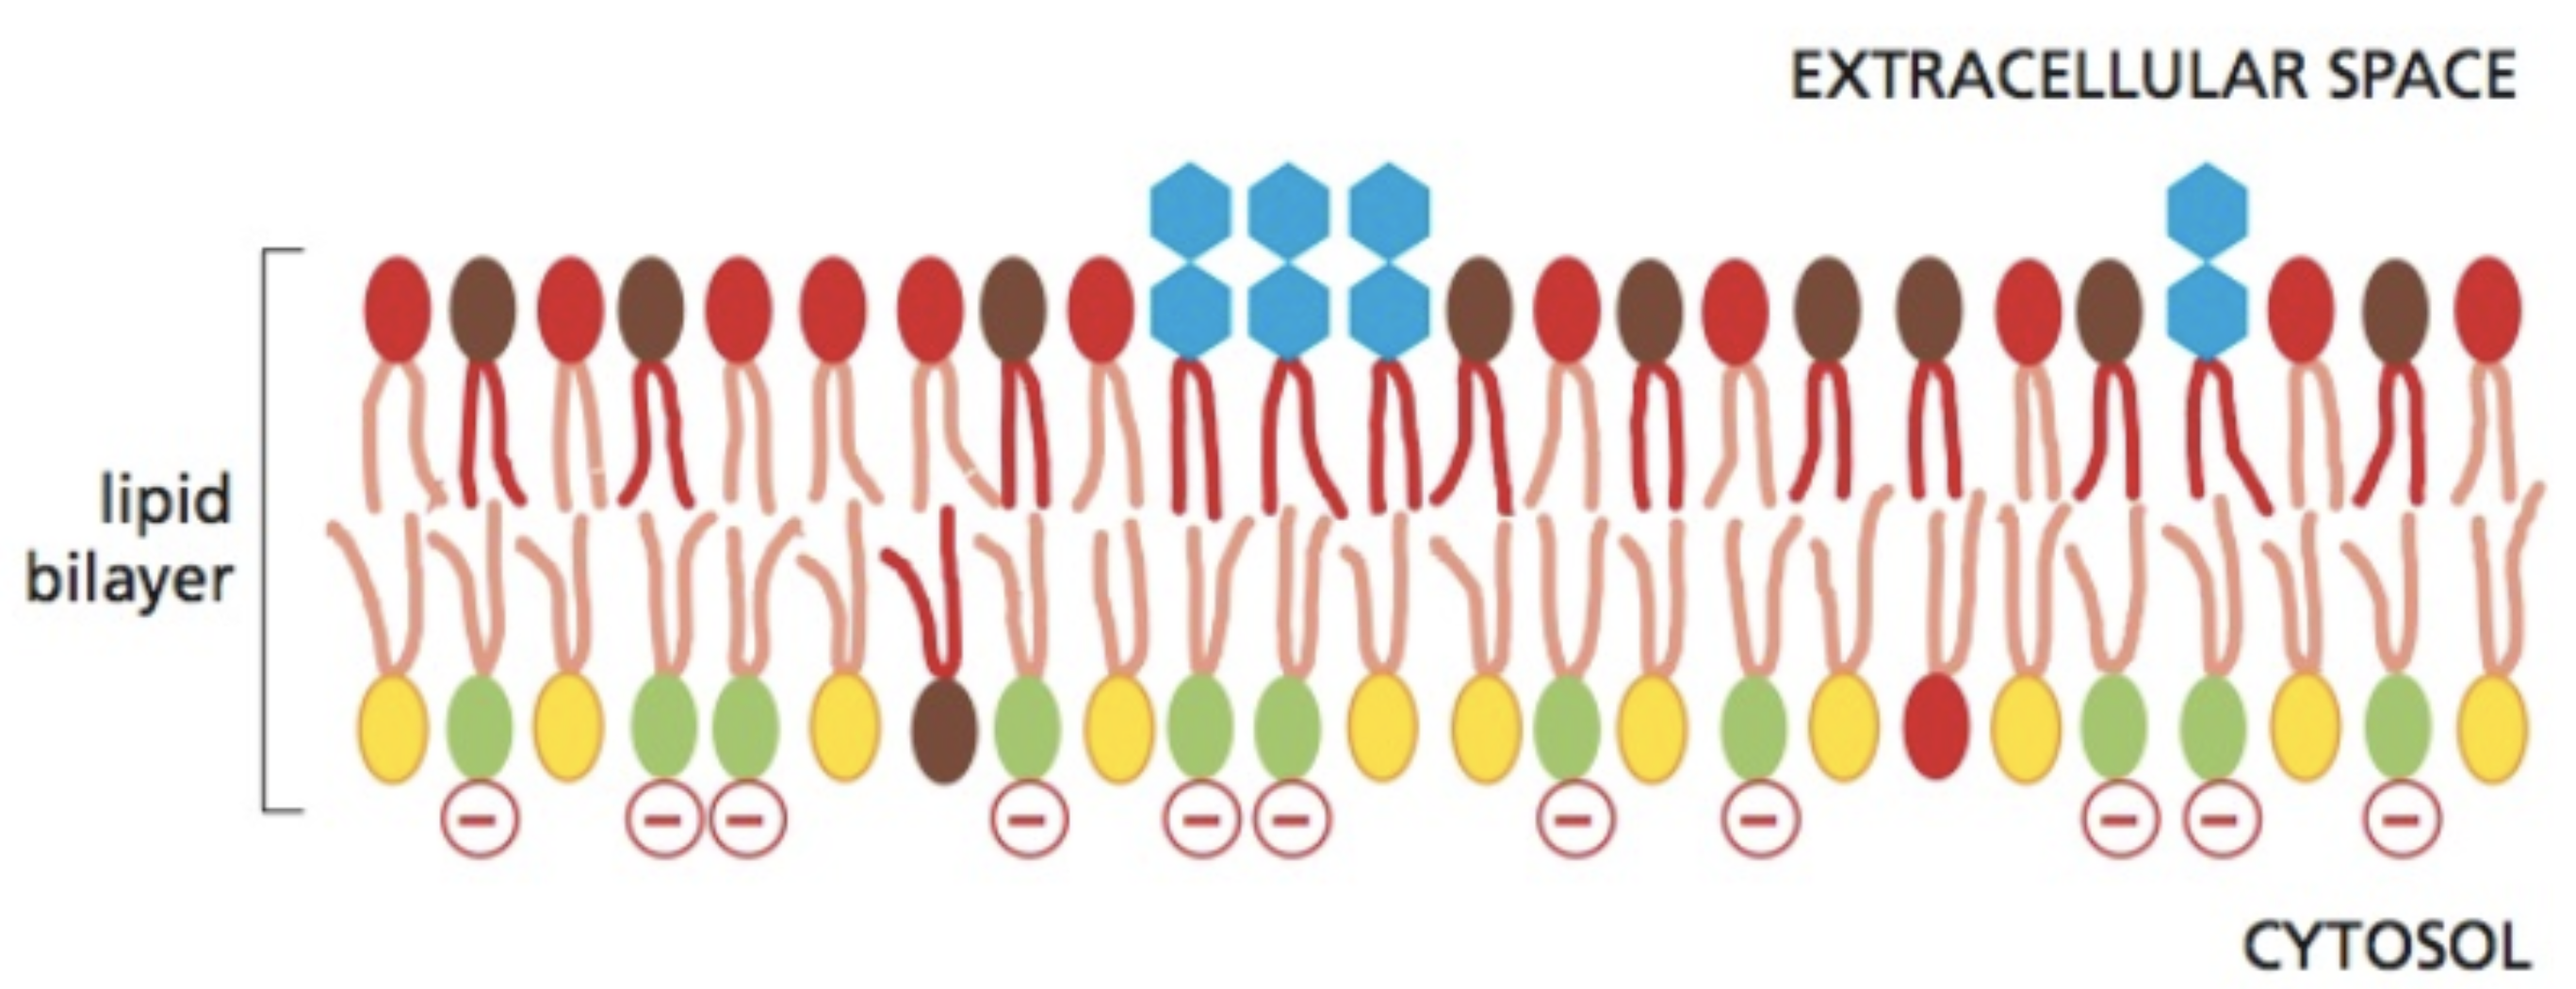
\includegraphics[width=0.4\linewidth]{../ExtFiles/plasmaMembraneAsyma.png}
            \caption{Phospholipid variations.}
            \label{fig:plasmaMembraneAsyma}
        \end{subfigure}
        \begin{subfigure}[b]{\linewidth}
            \centering
            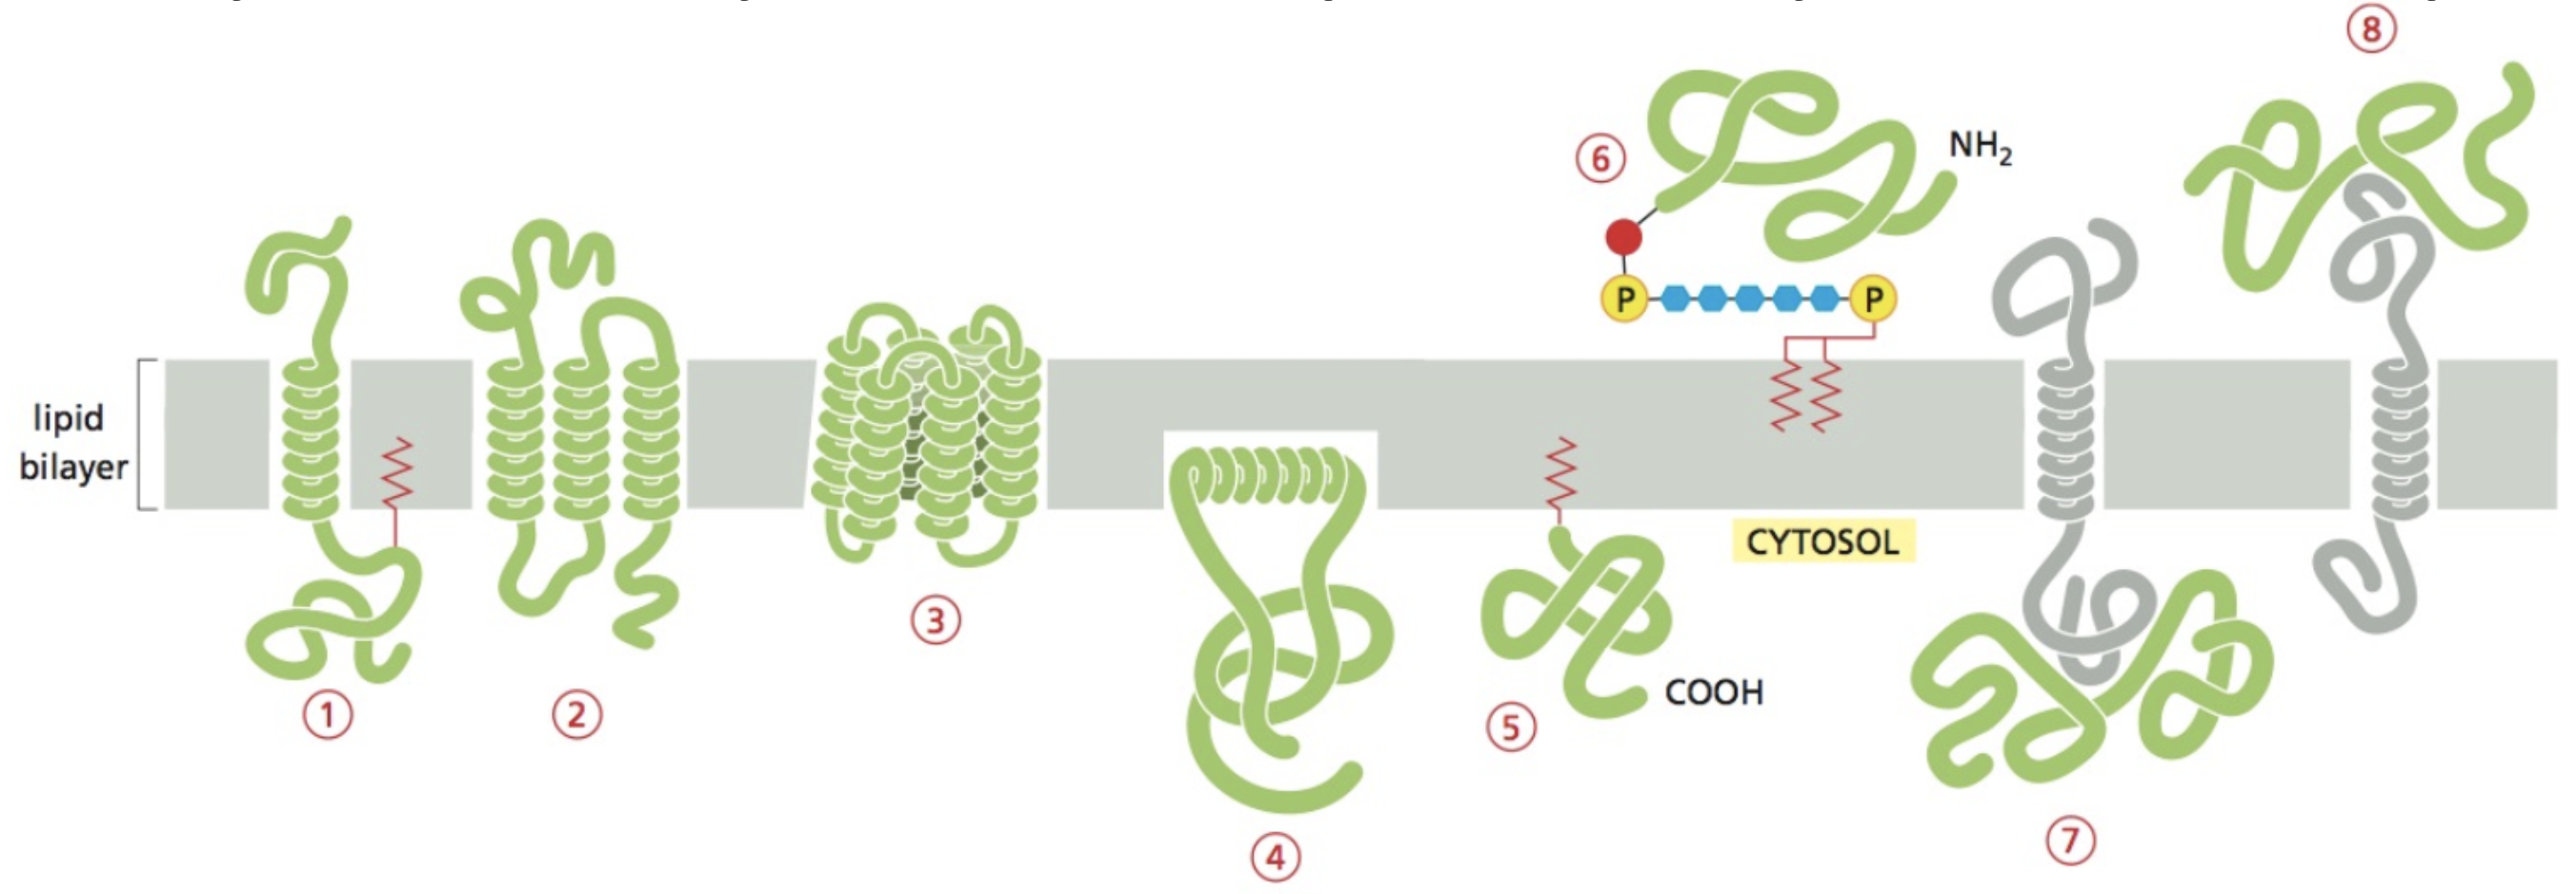
\includegraphics[width=0.7\linewidth]{../ExtFiles/plasmaMembraneAsymb.png}
            \caption{Membranous protein types.}
            \label{fig:plasmaMembraneAsymb}
        \end{subfigure}
        \caption{Asymmetry in the plasma membrane.}
        \label{fig:plasmaMembraneAsym}
    \end{figure}
    \begin{itemize}
        \item The outer and inner leaflets look quite different.
        \begin{itemize}
            \item Note that the four colors of phospholipids in Figure \ref{fig:plasmaMembraneAsyma} (red, brown, yellow, and green) correspond to the four head groups in Figure \ref{fig:plasmaMembraneConstituents}.
            \item The inner membrane has a lot of PS.
            \item The outer membrane has a lot of \textbf{glycolipids}.
        \end{itemize}
        \item If one head group has two tails, it looks like a cylinder. If one head group has multiple hydrophobic tails, it looks more like a cone. If one head group has a couple of tails and a large glycolipid, it will look like an inverted cone.
        \begin{itemize}
            \item This affects packing in the plasma membrane; larger hydrophilic groups need more space and cause the plasma membrane to pucker outwards; larger hydrophobic groups cause it to bend inwards.
        \end{itemize}
        \item We know a cell has died in the lab via annexin staining.
        \begin{itemize}
            \item When a cell is alive, it is constantly flipping PS molecules that have migrated to the outer leaflet back to the inner leaflet. When it dies, it can no longer do this, and PS molecules flip to the outer leaflet in large numbers.
            \item Annexins bind PS molecules, signaling to all immune cells that this one has died and they should come eat it.
        \end{itemize}
        \item Another place from which asymmetry comes is membranous proteins.
        \item Transmembrane proteins.
        \begin{itemize}
            \item Proteins can have transmembrane regions (usually $\alpha$-helical and hydrophobic).
            \item Some transmembrane proteins are \textbf{single-pass} while others are \textbf{multipass}.
            \item Once a transmembrane protein is synthesized, it folds, condensing and squeezing phospholipids that are in the way out of its volume.
        \end{itemize}
        \item Attaching a protein to the inner leaflet.
        \begin{itemize}
            \item Use an \textbf{amphipathic} helix.
            \item Proteins can also be \textbf{lipid anchored} to the membrane.
        \end{itemize}
        \item Protein-protein interactions with a single-pass transmembrane protein can attach proteins to the the inner or outer leaflet.
        \item Attaching a protein to the outer leaflet.
        \begin{itemize}
            \item Use a \textbf{GPI anchor}.
        \end{itemize}
    \end{itemize}
    \item \textbf{Glycolipid}: A huge number of sugars attached together to form a hydrophilic head group on the outside of the plasma membrane.
    \item \textbf{Single-pass} (transmembrane protein): A transmembrane protein that passes through the membrane once.
    \item \textbf{Multipass} (transmembrane protein): A transmembrane protein that passes through the membrane more than once, with the different transmembrane regions connected by various AA chain linkers.
    \item \textbf{Amphipathic} (helix): An $\alpha$-helix for which one side is hydrophilic and the other is hydrophobic.
    \begin{itemize}
        \item These are rare.
        \item They insert into the surface of the plasma membrane, with the hydrophilic region oriented toward the cytoplasm and the hydrophobic region oriented toward the hydrophobic interior of the plasma membrane.
    \end{itemize}
    \item \textbf{Lipid anchor}: A fatty acid lipid chain covalently bound to a protein and inserted into a cell's plasma membrane.
    \begin{itemize}
        \item Some proteins show out a serine, cysteine, or lysine. These are capable of being alkylated (via an ester, thioester, or amide linkage, respectively). The alkyl chain can then bind to a fatty acid lipid chain, which embeds itself in the similarly hydrophobic region of the plasma membrane.
        \item Single lipid anchors usually aren't very stable; in order to achieve stable integration, you typically need one more chain.
    \end{itemize}
    \item \textbf{GPI anchor}. \emph{Also known as} \textbf{Glycosylphosphatidylinositol anchor}, \textbf{GPI linker}.
    \begin{itemize}
        \item Very important.
        \item A protein attaches (via a GPI linker) to a lipid; we'll talk about these in greater depth later.
    \end{itemize}
    \item Different kinds of lipid anchors.
    \begin{figure}[h!]
        \centering
        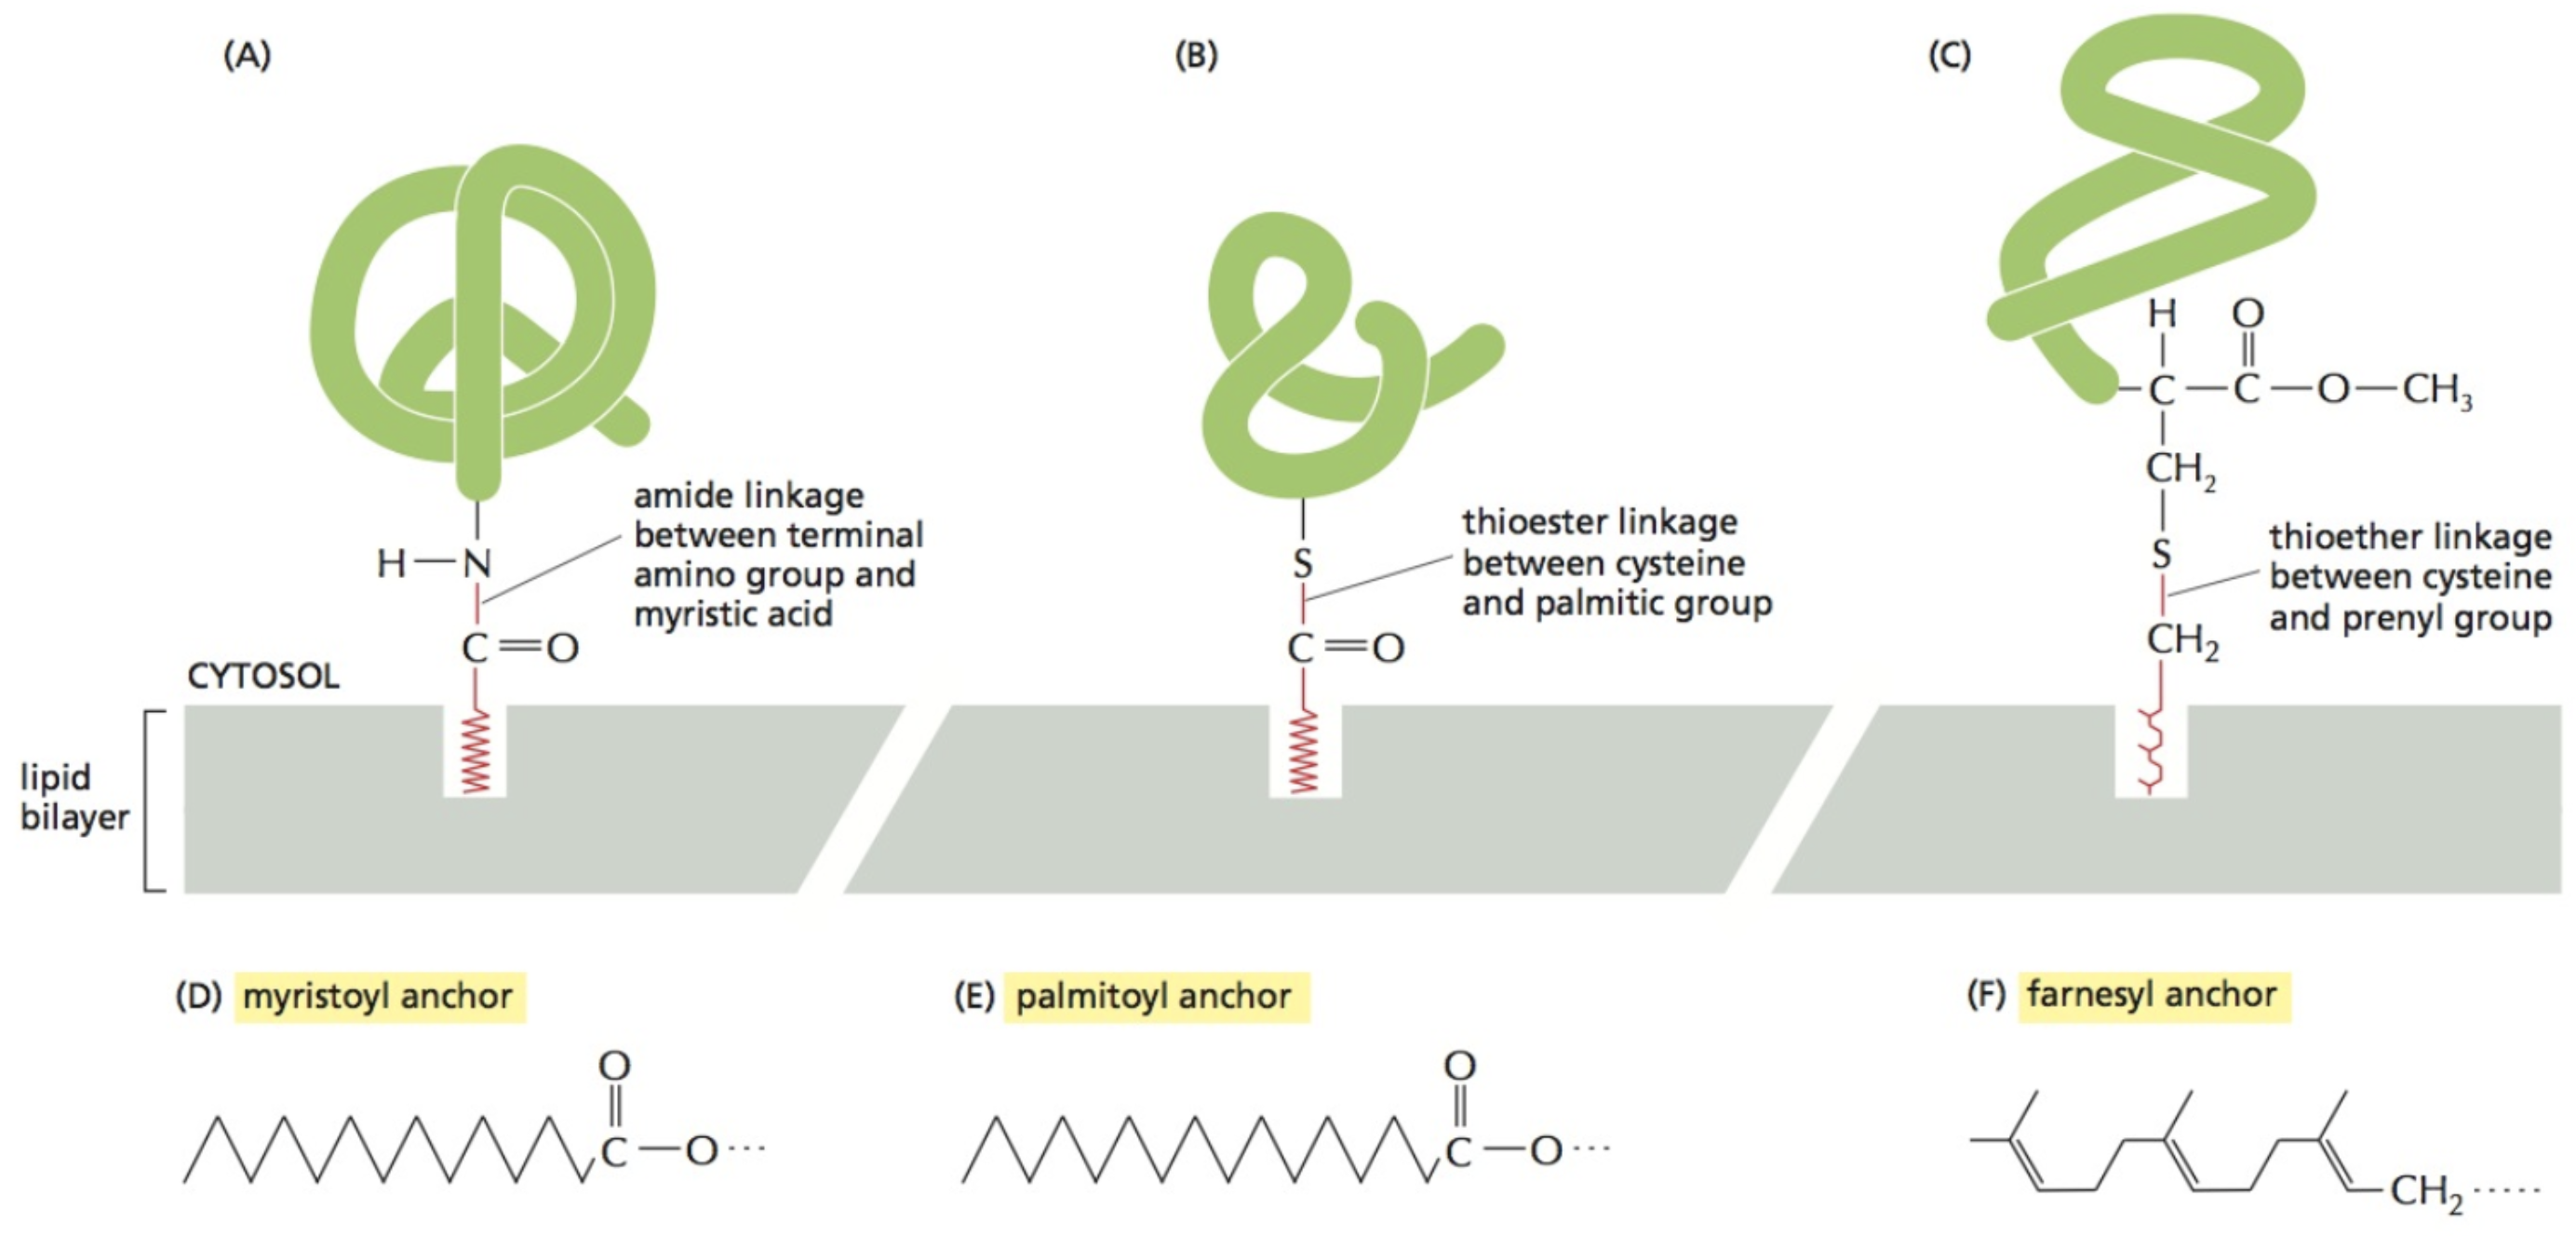
\includegraphics[width=0.7\linewidth]{../ExtFiles/lipidAnchorTypes.png}
        \caption{Lipid anchor types.}
        \label{fig:lipidAnchorTypes}
    \end{figure}
    \item Most transmembrane proteins cross the bilayer in an $\alpha$-helical conformation.
    \begin{figure}[H]
        \centering
        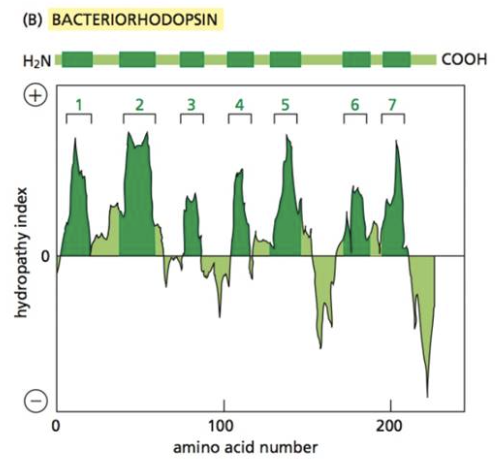
\includegraphics[width=0.4\linewidth]{../ExtFiles/hydropathyChart.png}
        \caption{Hydropathy chart example.}
        \label{fig:hydropathyChart}
    \end{figure}
    \begin{itemize}
        \item Transmembrane domains are predicted using the \textbf{hydropathy index}.
        \item You use a sliding window of 20 AAs. This means that you average the hydropathy indices of 20 adjacent amino acids at a time in a protein to determine what 20-AA region has the highest overall hydropathy index. This region is the one that's most likely to be transmembrane.
        \item From a plot of the sliding window hydrophobicity vs. AA number, you can look for peaks in hydrophobicity. These correspond to hydrophobic, transmembrane regions.
        \begin{itemize}
            \item There will be a question about this in the exam!
        \end{itemize}
    \end{itemize}
    \item \textbf{Hydropathy index}: The amount of Gibbs free energy needed to transfer an amino acid residue from water to a nonpolar solvent.
    \begin{itemize}
        \item A positive value means that the AA is hydrophobic; vice versa if the value is negative.
    \end{itemize}
    \item Most transmembrane proteins cross the bilayer in an $\alpha$-helical conformation.
    \begin{figure}[h!]
        \centering
        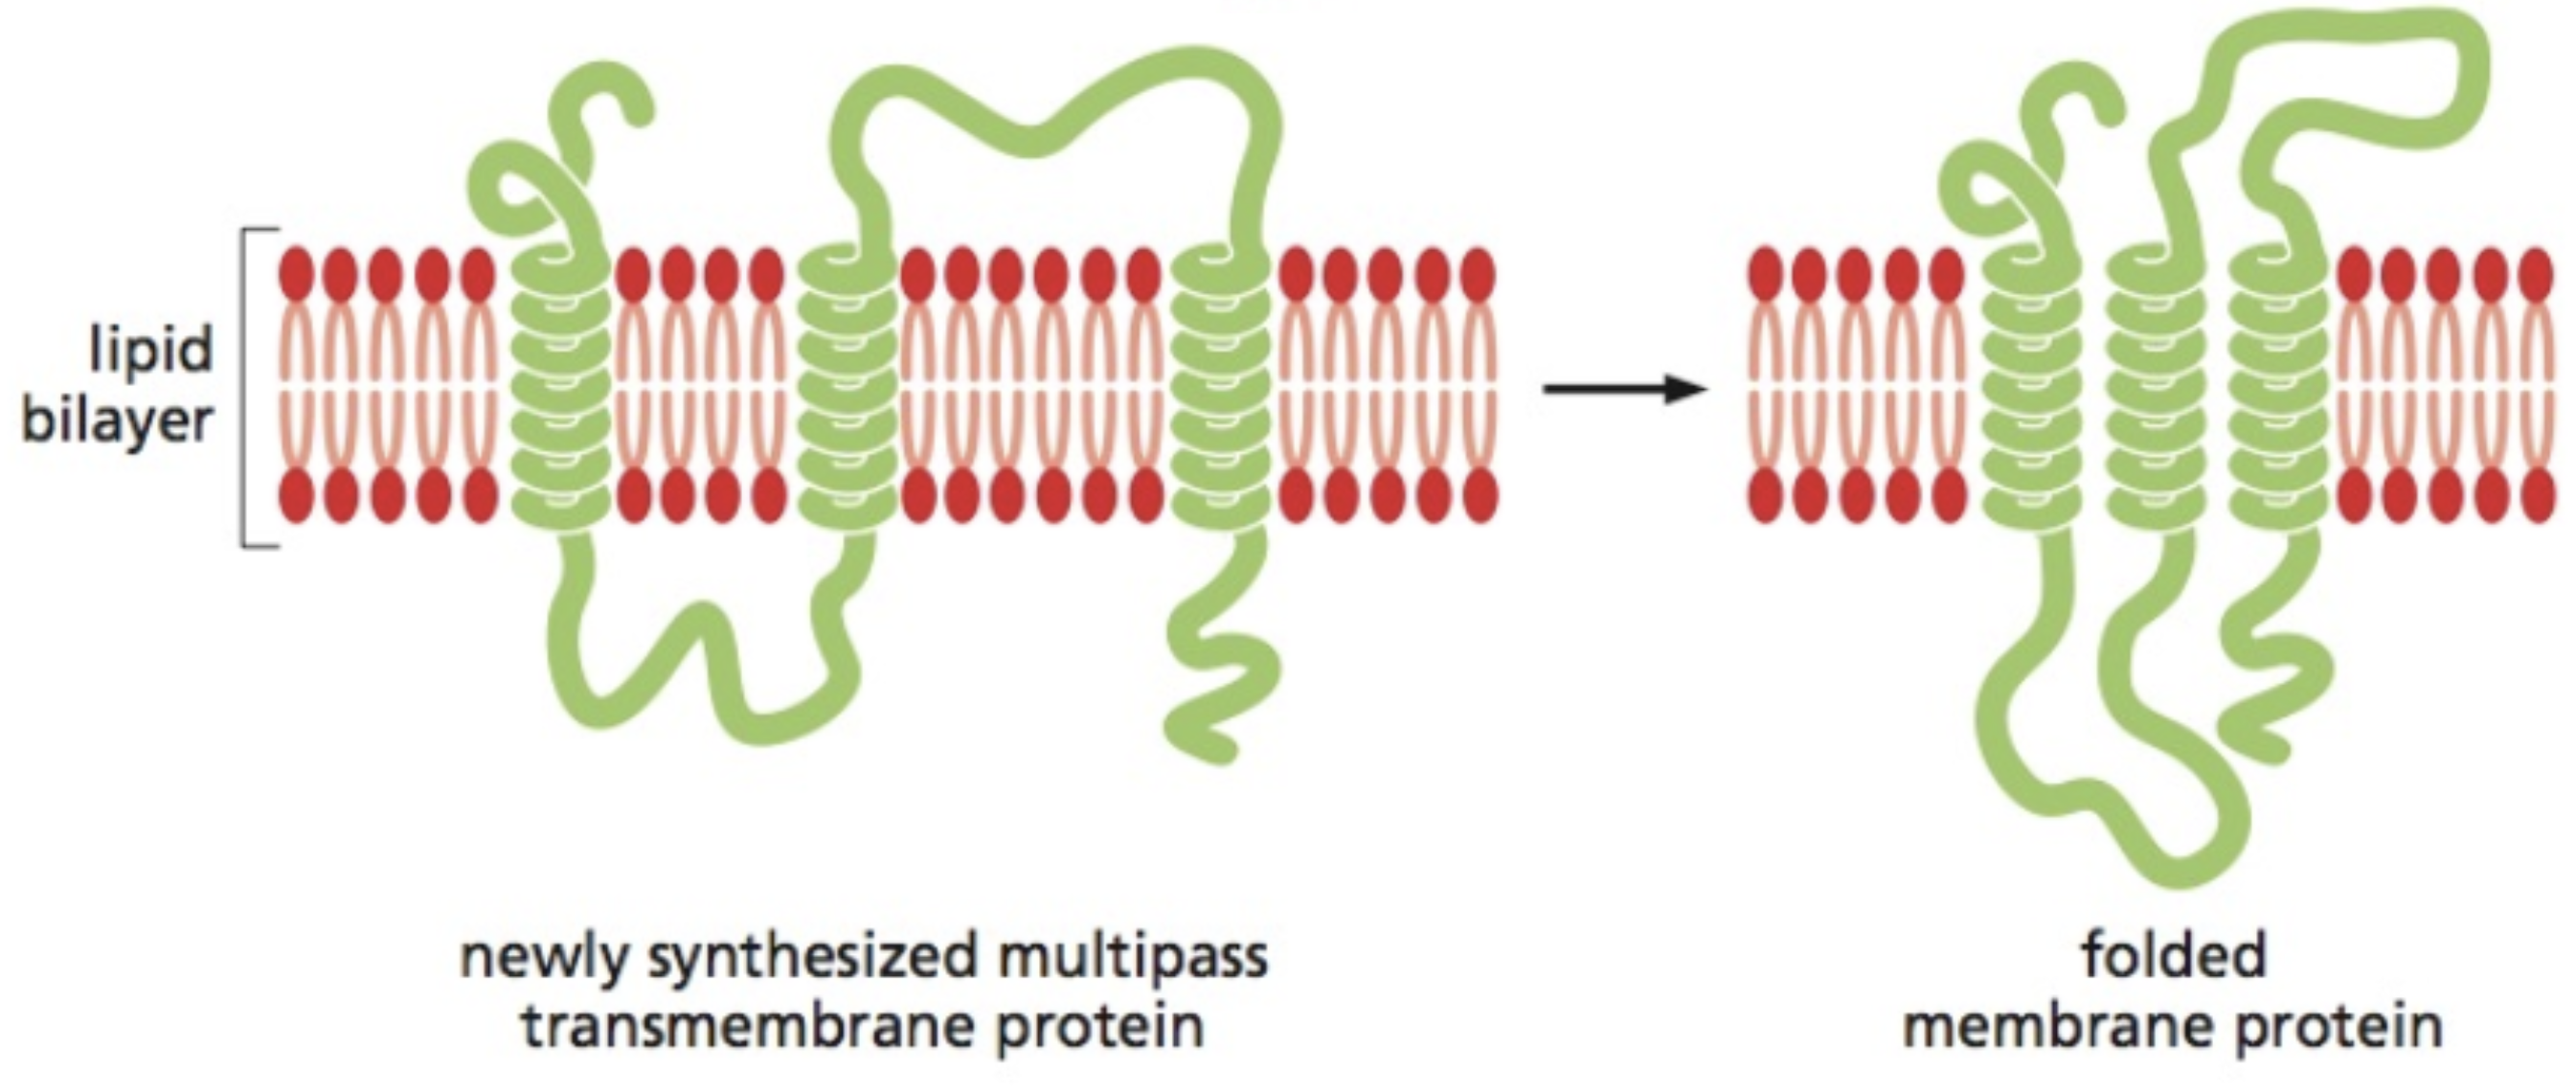
\includegraphics[width=0.4\linewidth]{../ExtFiles/multipassFolding.png}
        \caption{Multipass transmembrane protein folding.}
        \label{fig:multipassFolding}
    \end{figure}
    \begin{itemize}
        \item As a protein is produced (more on production in the ER and transport to the cell surface later), the transmembrane domains insert into the plasma membrane and squeeze out intermediate phospholipids.
    \end{itemize}
    \item Proteins are embedded in different ways.
    \begin{figure}[h!]
        \centering
        \begin{subfigure}[b]{\linewidth}
            \centering
            \includegraphics[width=0.4\linewidth]{../ExtFiles/alternateProteinEmbeddinga.png}
            \caption{$\beta$-barrel proteins.}
            \label{fig:alternateProteinEmbeddinga}
        \end{subfigure}\\[1em]
        \begin{subfigure}[b]{\linewidth}
            \centering
            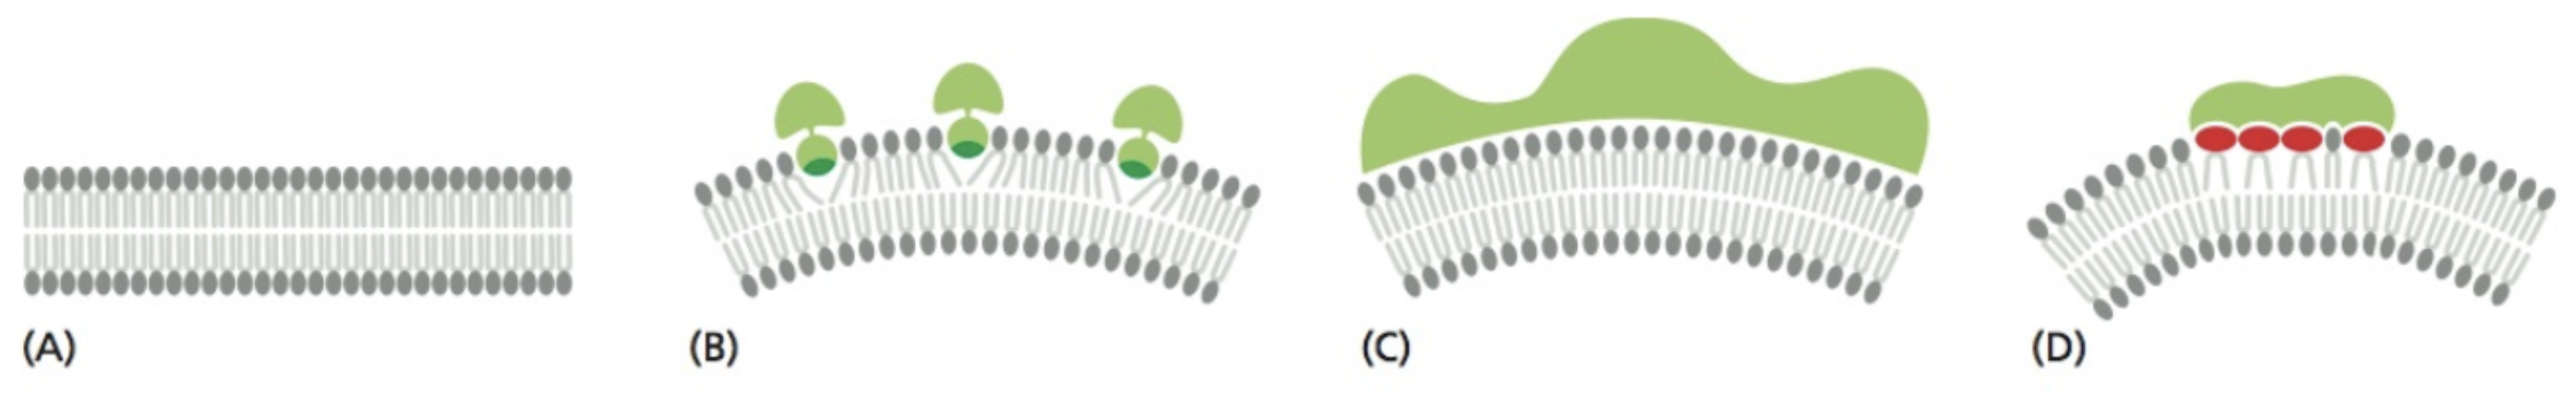
\includegraphics[width=0.7\linewidth]{../ExtFiles/alternateProteinEmbeddingb.png}
            \caption{Extracellular protein binding and resultant plasma membrane bending.}
            \label{fig:alternateProteinEmbeddingb}
        \end{subfigure}
        \caption{Alternate transmembrane protein embedding.}
        \label{fig:alternateProteinEmbedding}
    \end{figure}
    \begin{itemize}
        \item It is possible to embed without $\alpha$-helices. Indeed, we can use $\beta$-sheets composed of hydrophobic residues.
        \begin{itemize}
            \item Cytosolic proteins of this form tuck all of their hydrophobic side chains inside.
            \item Transmembrane proteins of this form show all of their hydrophobic side chains outside.
        \end{itemize}
        \item Example: The MSPA porin from nanopore sequencing.
        \item These are called \textbf{$\bm{\beta}$-barrel proteins} and are often involved in transport or are receptors.
        \item Barrel size varies.
        \begin{itemize}
            \item MSPA has a huge barrel.
            \item Smaller barrels are often filled up by amino acids on the inside but can act as a scaffold to interact with proteins on the top or bottom. Moreover, selected small molecules can sometimes pass through.
        \end{itemize}
        \item These channels are very large in general and can bend membranes by binding proteins on the outer leaflet.
        \begin{itemize}
            \item These can act as large head groups and induce outward puckering.
            \item A conformational change in the protein induced upon binding can place mechanical pressure on the membrane.
            \item A protein can bind to multiple head groups and push them apart.
        \end{itemize}
    \end{itemize}
    \item The inside vs. the outside of the cell.
    \begin{itemize}
        \item 33\% of our ATP goes to maintaining ion gradients.
        \item Remember that some molecules are rich outside and poor inside, and vice versa.
        \item For example, cells need to take in glucose and enrich its concentration within the cell.
    \end{itemize}
    \item We now look at the transport processes that maintain these gradients.
    \item There are two main classes of membrane transport proteins.
    \begin{figure}[h!]
        \centering
        \begin{subfigure}[b]{0.49\linewidth}
            \centering
            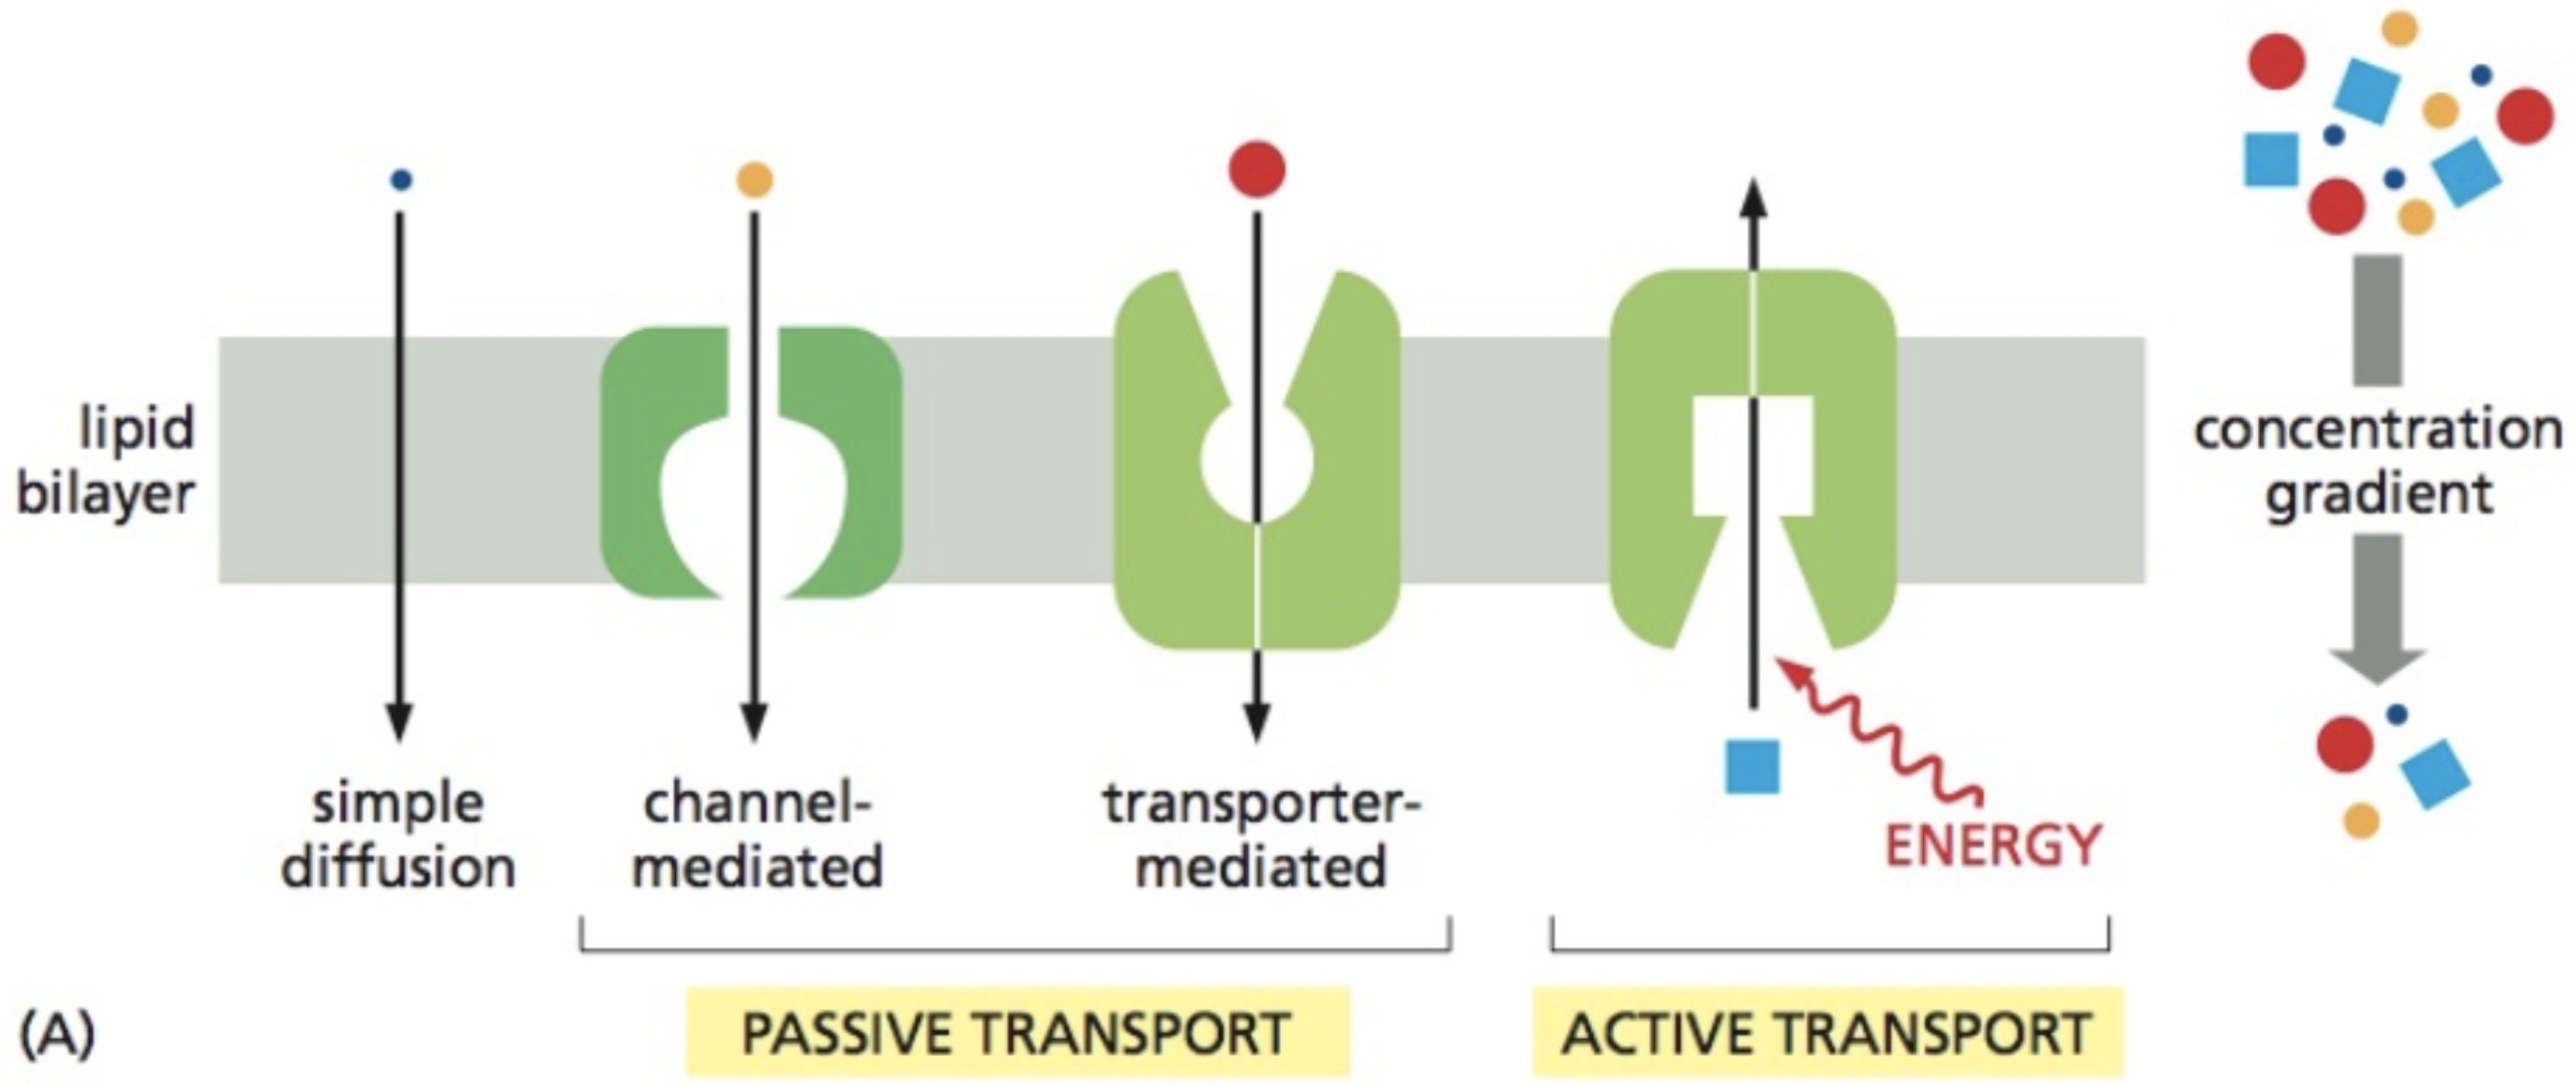
\includegraphics[width=0.9\linewidth]{../ExtFiles/transportTypesa.png}
            \caption{Types of transport.}
            \label{fig:transportTypesa}
        \end{subfigure}
        \begin{subfigure}[b]{0.49\linewidth}
            \centering
            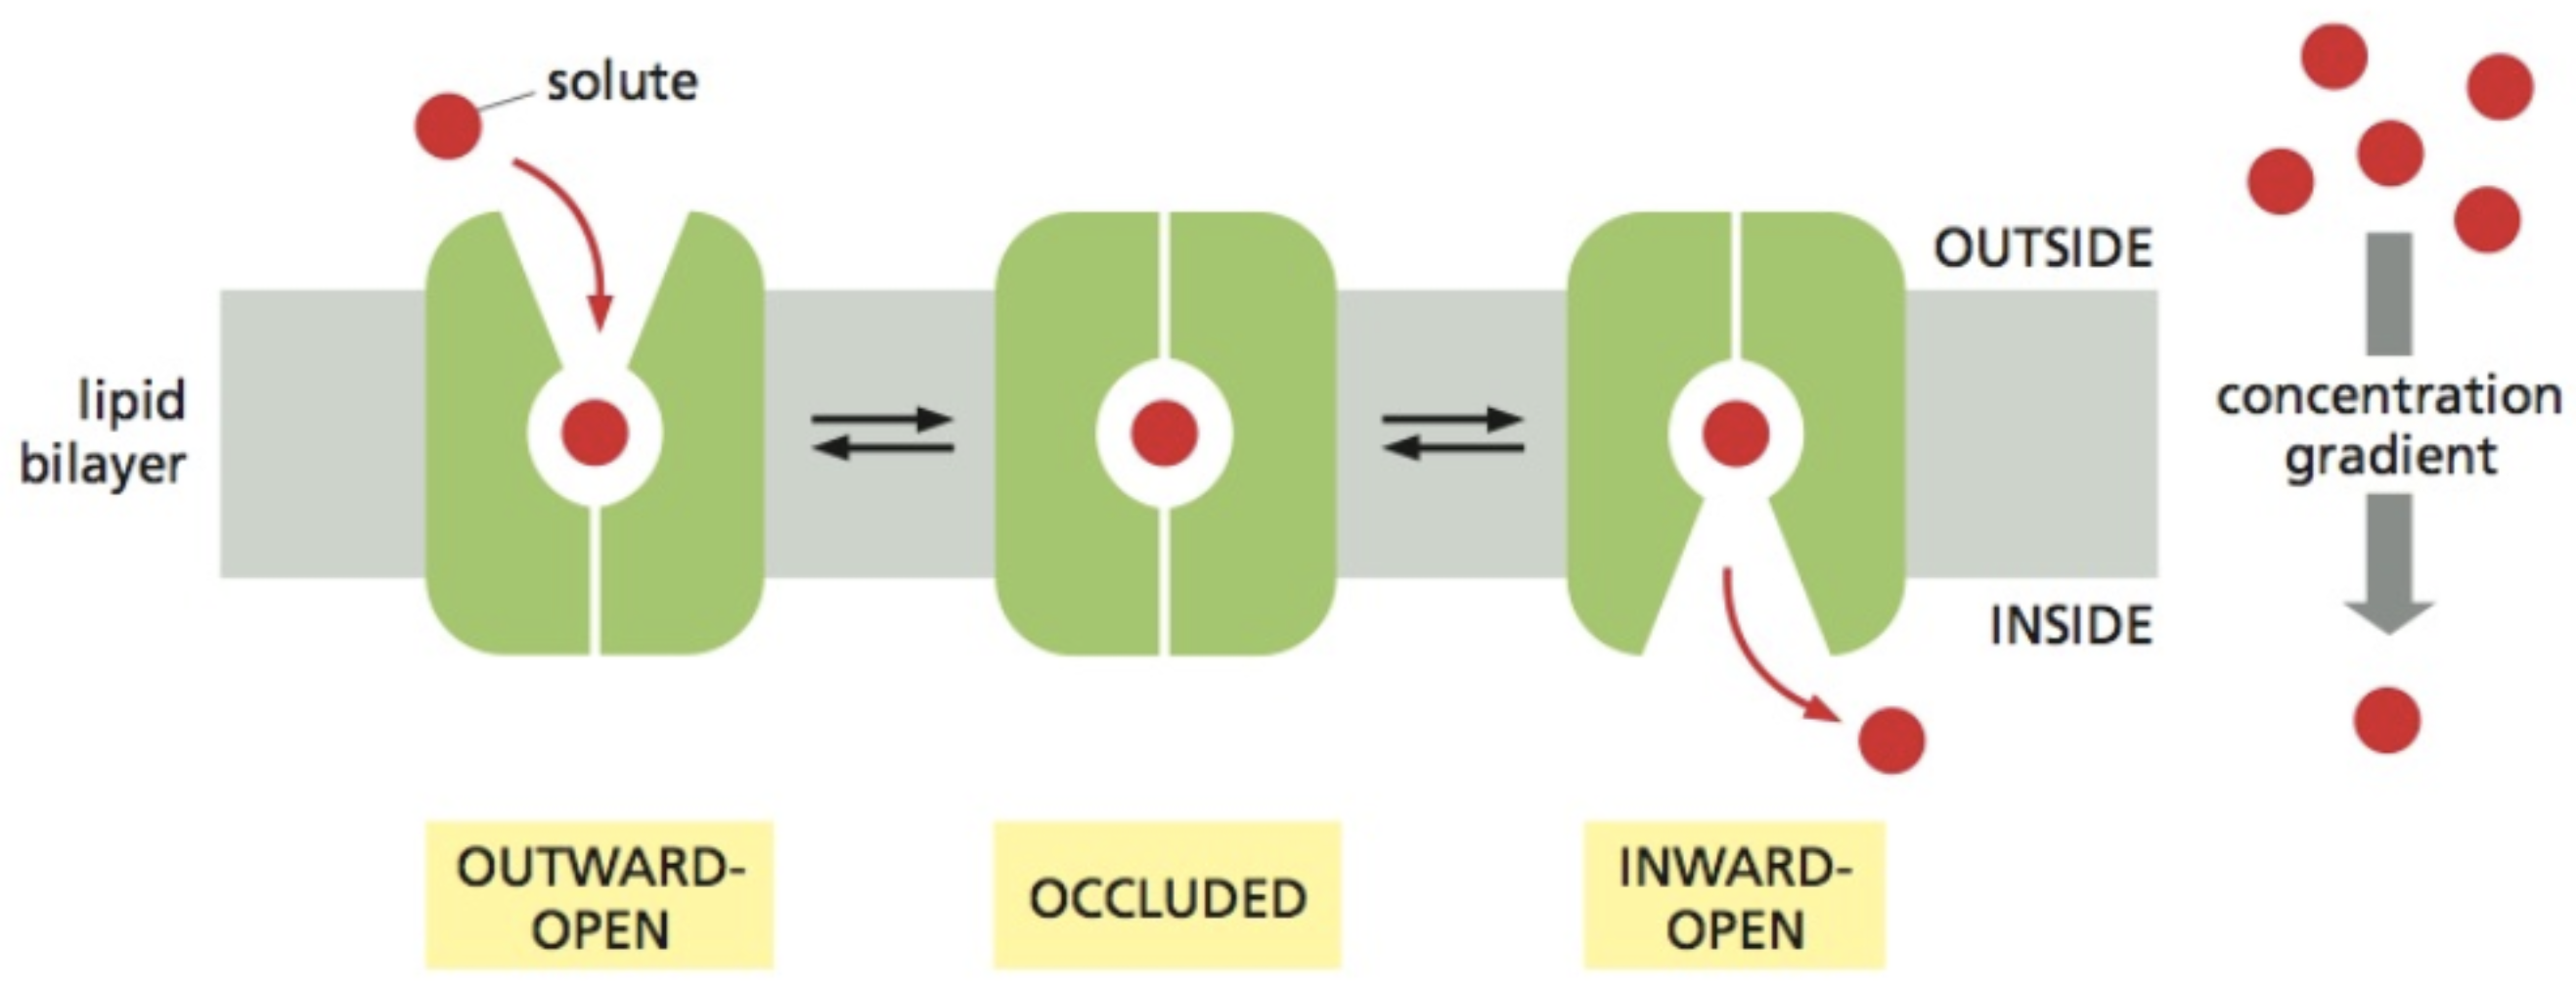
\includegraphics[width=0.9\linewidth]{../ExtFiles/transportTypesb.png}
            \caption{Phases of transporter-mediated passive transport.}
            \label{fig:transportTypesb}
        \end{subfigure}
        \caption{Membrane transport options.}
        \label{fig:transportTypes}
    \end{figure}
    \begin{itemize}
        \item \textbf{Passive transport} vs. \textbf{active transport}.
        \item Types of passive transport: There is some simple diffusion/leakage, channel-mediated diffusion such as ion channels allow very fast diffusion, and transporter-mediated diffusion to move larger molecules.
        \item Transporters usually catch molecules on one side of the membrane, inducing a conformational change, and release them on the other side of the membrane. Outward-open, occluded, and inward-open states.
    \end{itemize}
    \item \textbf{Passive transport}: A type of membrane transport that \emph{does not} require energy to move substances across cell membranes.
    \item \textbf{Active transport}: A type of membrane transport that \emph{does} require energy to move substances across cell membranes.
    \item How a cell regulates concentration gradients.
    \begin{figure}[h!]
        \centering
        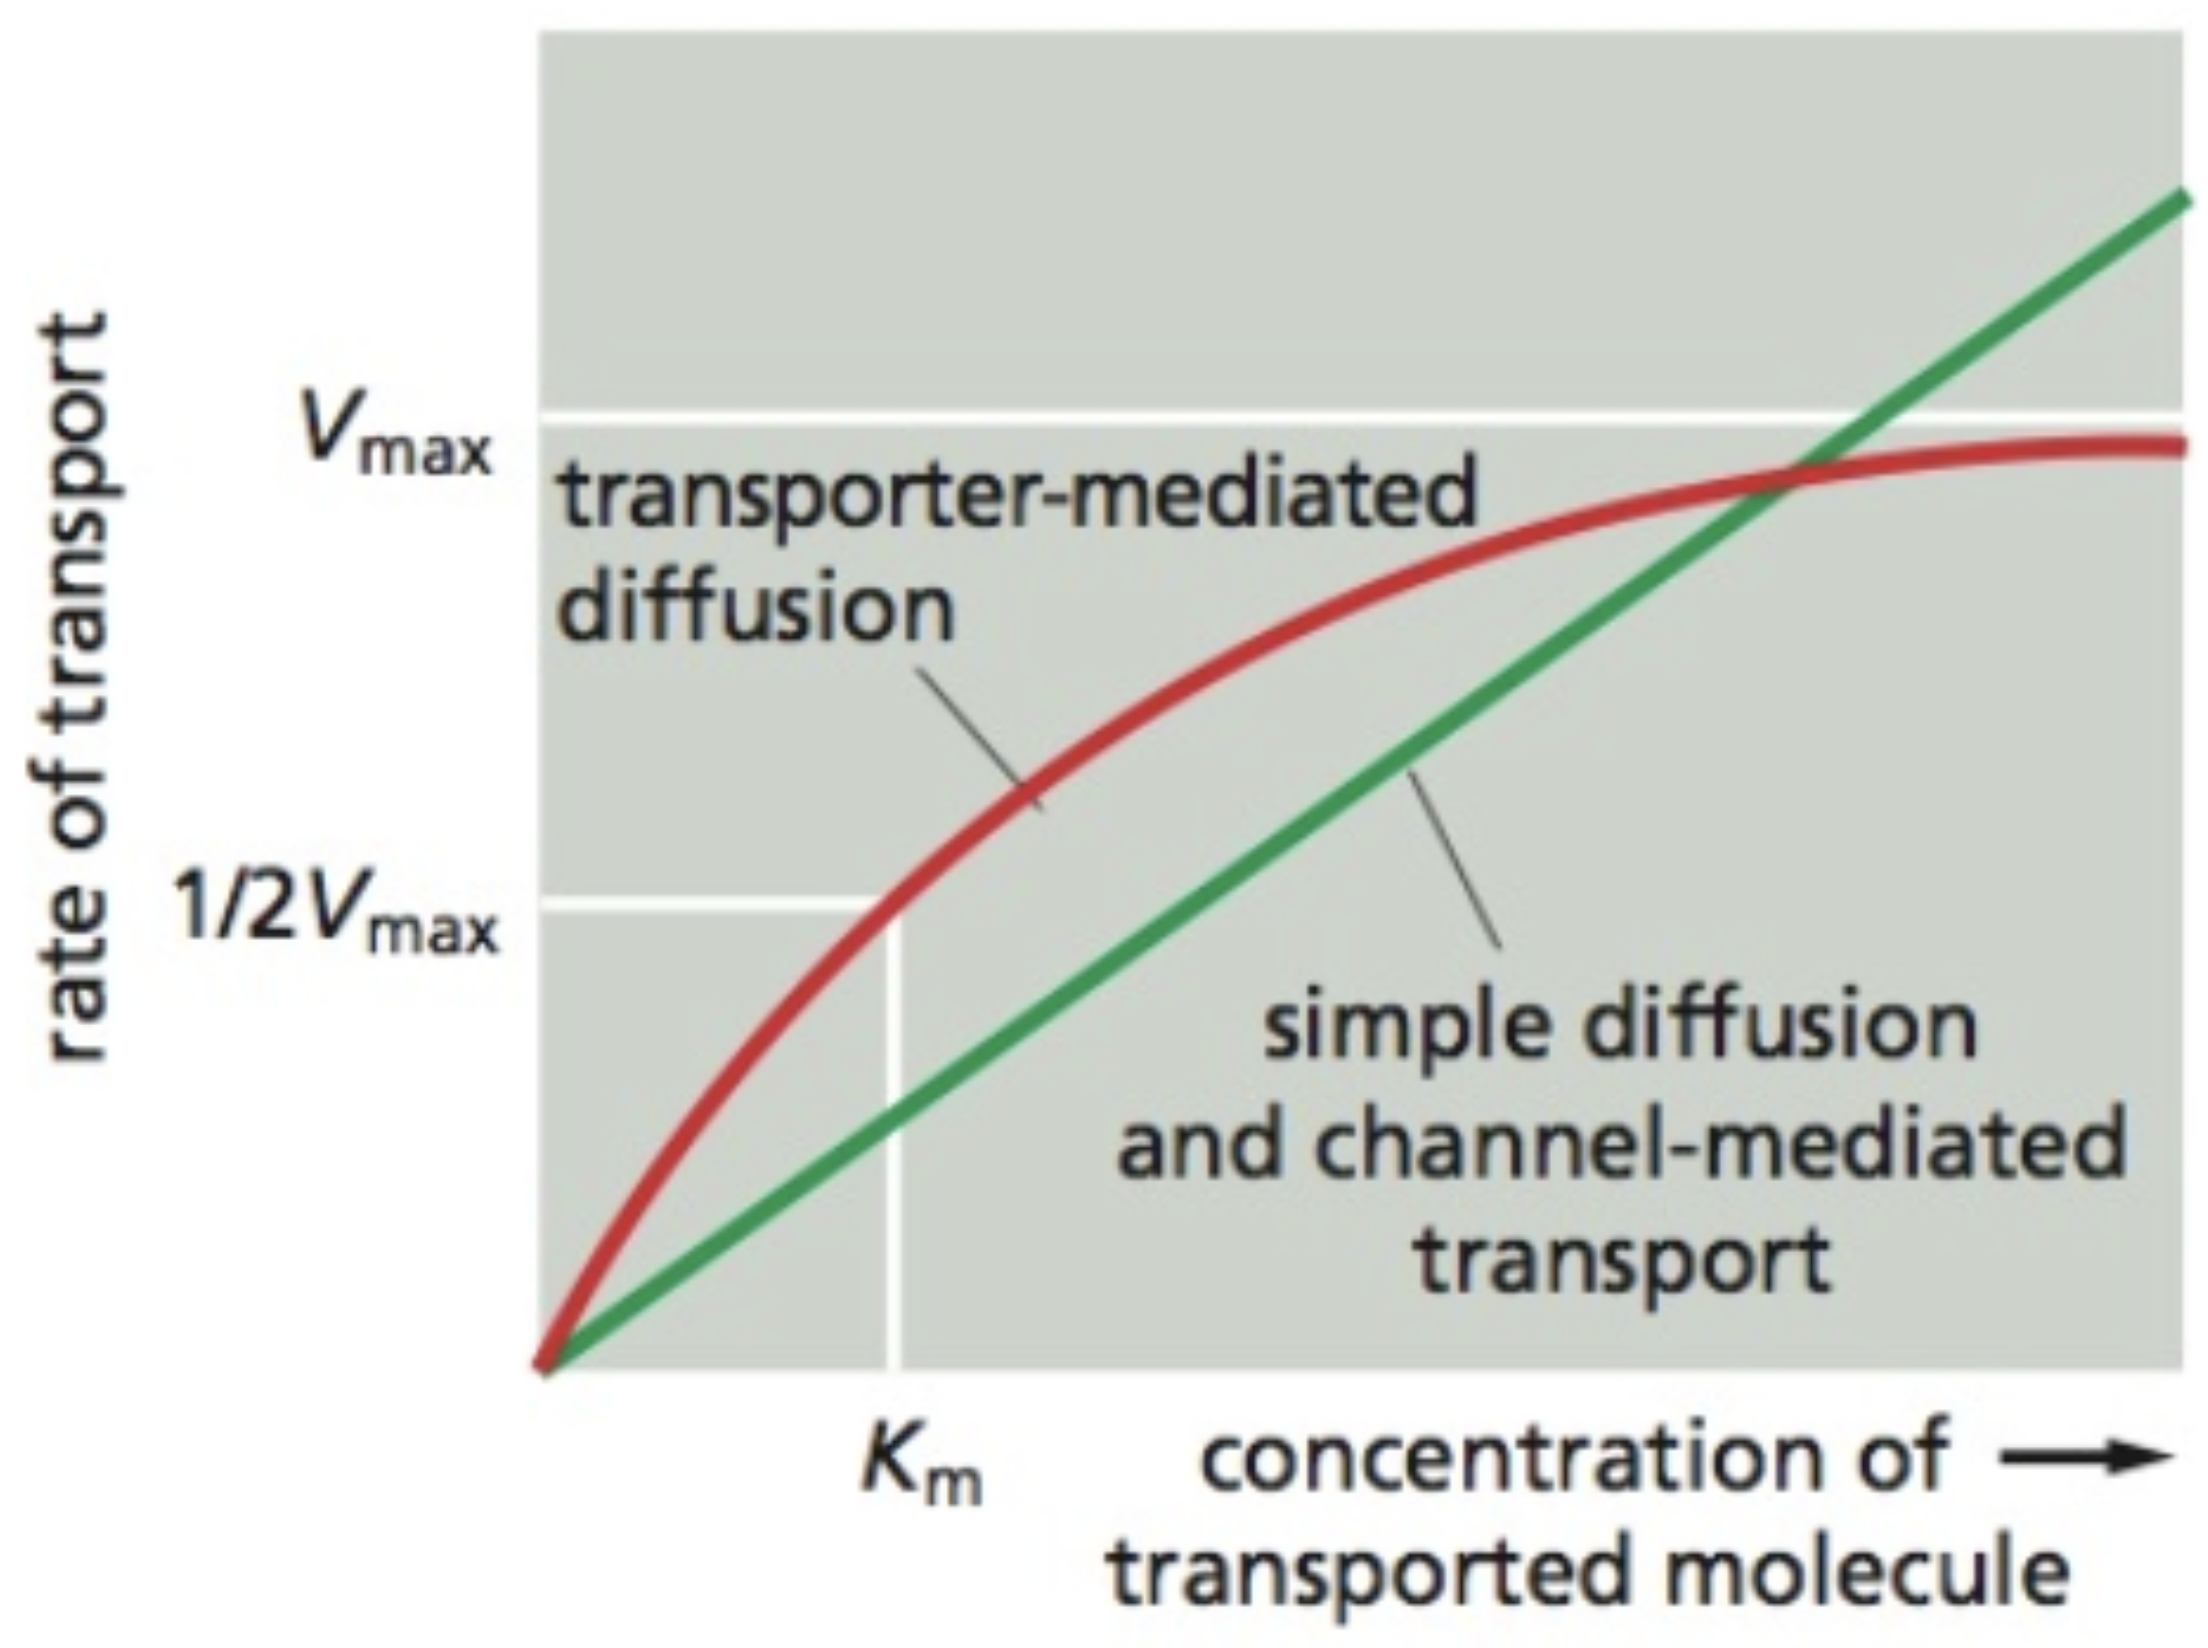
\includegraphics[width=0.33\linewidth]{../ExtFiles/concentrationGradientRegulation.png}
        \caption{Concentration gradient regulation.}
        \label{fig:concentrationGradientRegulation}
    \end{figure}
    \begin{itemize}
        \item As per the Michaelis-Menten mechanism, transporter-mediated diffusion starts out strong but eventually levels out at some $v_\text{max}$ as the concentration of the transported molecule increases.
        \item Simple diffusion and channel-mediated transport, however, increase linearly with the concentration of transported molecule indefinitely.
        \item Thus, equilibrium is established when the rate of transporter-mediated diffusion in one direction equals the rate of simple diffusion and channel-mediated transport in the other direction (the intersection of the two lines on the right of Figure \ref{fig:concentrationGradientRegulation}).
    \end{itemize}
    \item Types of transporters.
    \begin{itemize}
        \item Most transporters are \textbf{coupled transporters}.
        \item Another kind is \textbf{ATP-driven pumps}.
        \item Energy can also come from light, as in \textbf{light-driven pumps}.
    \end{itemize}
    \item \textbf{Coupled transporter}: A transporter that moves two molecules either in the same or opposite directions. \emph{Also known as} \textbf{cotransporter}.
    \begin{itemize}
        \item \textbf{Symporters} and \textbf{antiporters} are the two types of coupled transporters.
    \end{itemize}
    \item \textbf{ATP-driven pump}: The ATPase domain hydrolyzes ATP, providing energy to power a conformational change that allows binding and then transport from low concentration to high concentration.
    \item \textbf{Light-driven pump}: The energy for the conformational change comes from light instead of ATP.
    \item \textbf{Uniporter}: A transporter that only moves a single kind of entity.
    \item \textbf{Symporter}: A transporter that moves two different entities in the same direction.
    \begin{itemize}
        \item Example: Transporting glucose using sodium. You need sodium as a co-transported ion to transport glucose.
    \end{itemize}
    \item \textbf{Antiporter}: A transporter that alternates between taking one molecule into the cell and another out.
    \item An example of coupled transport: The sodium-coupled glucose transporter's steps.
    \begin{figure}[h!]
        \centering
        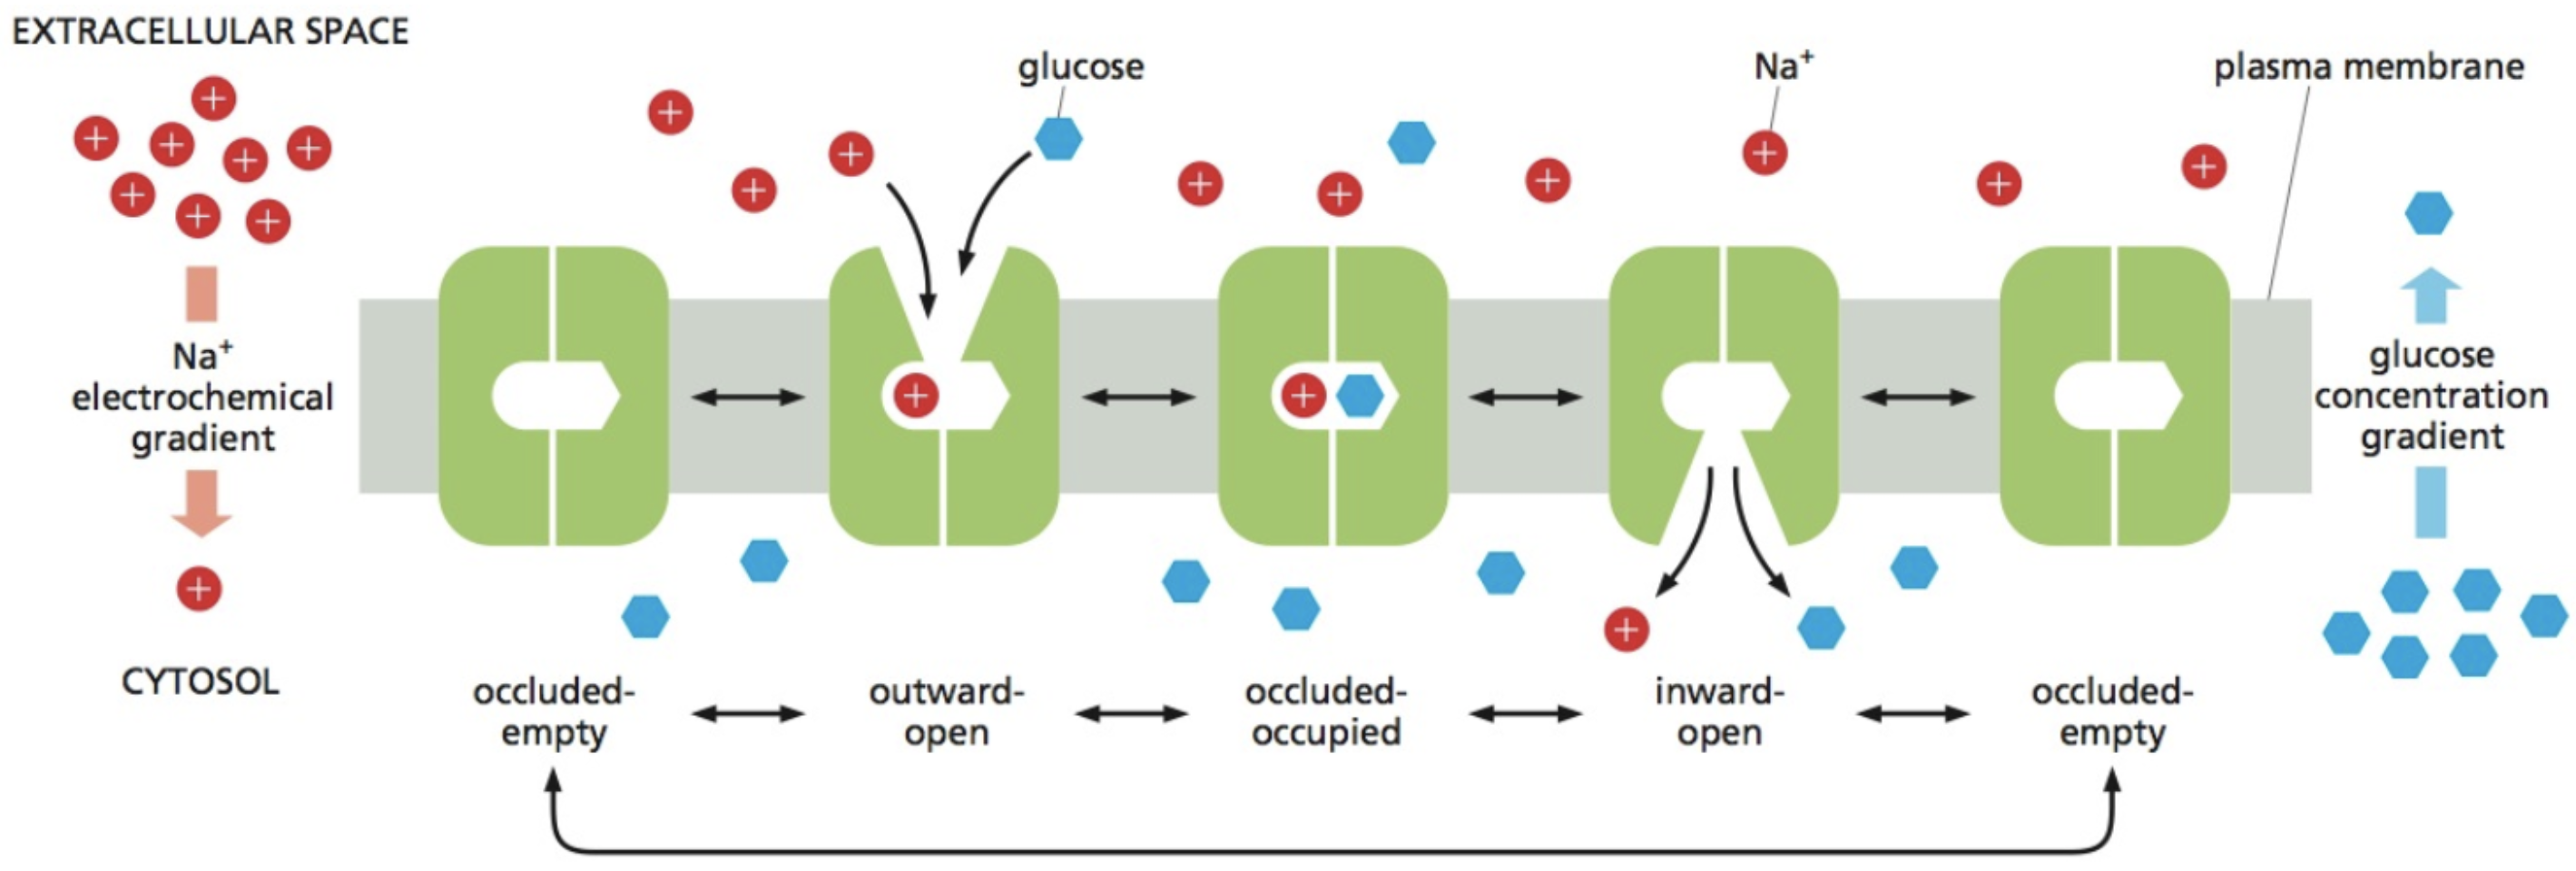
\includegraphics[width=0.7\linewidth]{../ExtFiles/NaGlucoseTransp.png}
        \caption{Sodium-glucose cotransporter activity.}
        \label{fig:NaGlucoseTransp}
    \end{figure}
    \begin{enumerate}
        \item Occluded-empty.
        \item Outward-open. Sodium has a high $K_d$, so it binds readily. This induces a conformational change, generating a high-affinity glucose-binding site.
        \item Occluded-occupied.
        \item Inward-open. Sodium falls off first. This induces a conformational change, removing the high-affinity glucose-binding site and kicking glucose out.
        \item Repeat.
    \end{enumerate}
    \item Key thing to remember about the plasma membrane: We tend to think of cells like HELA cells and HEK cells that are apolar, but real cells do have poles and specific regions with fundamentally different membranes.
    \begin{itemize}
        \item For example, consider intestinal cells (I-cells). One side faces the gut and all of the bacteria therein (we are 98\% bacteria by number of cells), the opposite side faces our vasculature (bloodstream) for easy deposition of nutrients, and the sides are bound to each other with protein velcro to keep the bacteria from getting into our blood (which would cause sepsis).
    \end{itemize}
    \item In addition to directly inhibiting proteins, you can simply stop them from going where they need to, e.g., if you want to inactivate a transmembrane protein, simply stopping it from leaving the ER and getting to the plasma membrane will do the job.
    \item The bending of membranes allows very similar chemical structures to achieve different objectives on a "macro" scale.
    \begin{itemize}
        \item Only 2-5\% of total cell membrane is the plasma membrane.
        \item Mitochondria contain a long, smooth, ellipsoidal outer membrane.
        \item Mitochondria also contain a long, fenestrated inner membrane.
        \item The endoplasmic reticulum's membrane has both flat and tubular regions. We don't know how the balance is decided, though.
    \end{itemize}
    \item \textbf{Solute liquid carriers} (SLCs) sit on the cell surface and are involved in nutrient transport. Every SLC mutation results in a different disease. These are symporters. These are the next class of druggable molecules.
    \item What is the purpose of aquaporins?
    \begin{itemize}
        \item These control the membrane tension, which is critical.
        \item Work together with sodium and potassium transporters.
    \end{itemize}
    \item Cystic fibrosis isn't concerned with water pressure; it's concerned with chloride concentration.
    \begin{itemize}
        \item Yamuna's advice: If you want to lose weight, stop eating salt. Low external salt gradients make it harder to transport amino acids into cells.
    \end{itemize}
\end{itemize}



\section{Supplementary Sequencing Videos}
\subsection*{PCR}
\emph{From \href{https://youtu.be/iQsu3Kz9NYo}{here}.}
\begin{itemize}
    \item \marginnote{11/9:}Denaturation temperature (for splitting DNA strands): \SI{95}{\celsius}.
    \item \textbf{Annealing} temperature (for binding primers to ssDNAs): \SIrange{55}{65}{\celsius}.
    \item Extension temperature (for DNA replication): \SI{72}{\celsius}.
    \item \textbf{DNA annealing}: The process of forming heteroduplex DNA from two complementary (or nearly complementary) molecules or regions of ssDNA. \emph{Also known as} \textbf{hybridizing}.
    \item From one single DNA molecule, 1,073,741,764 copies of the target DNA are obtained in only 4 hours.
\end{itemize}


\subsection*{Pyrosequencing}
\emph{From \href{https://youtu.be/CdHTLLF-abA}{here}.}
\begin{itemize}
    \item First, we need a strand of DNA to sequence
    \item Step 1: Make the \textbf{library}.
    \begin{itemize}
        \item Cut the DNA into fragments via \textbf{sonication} or \textbf{nebulization}.
        \item Then the fragmented DNA strands are ligated with \textbf{adapters} at both the $5'$ and $3'$ ends.
        \item At this point, we denature the dsDNA, generating a hybrid molecule that we can amplify with PCR in step 2.
    \end{itemize}
    \item \textbf{Library}: A collection of DNA fragments that we store and clone.
    \item \textbf{Sonication}: A technique of shearing DNA involving exposing it to high sound frequencies to agitate it and cause it to break.
    \item \textbf{Nebulization}: A technique of shearing DNA involving forcing it through a small hole.
    \item \textbf{Adapter}: A short oligonucleotide.
    \item \textbf{Oligonucleotide}: A short single- or double-stranded DNA or RNA molecule. \emph{Also known as} \textbf{oligo}.
    \item Step 2: Emulsion PCR.
    \begin{itemize}
        \item We incubate the DNA with microscopic beads that are bound all around with oligos complementary to our adapters.
        \item Thus, every ssDNA can anneal to the DNA capture beads.
        \item Subsequent dilution ensures that each bead only has one strand attached.
        \item Oil is added to the mixture forming an \textbf{emulsion} with the largely aqueous solvent.
        \item This creates \textbf{blebs}.
        \item We add a PCR mix (buffer, primer, polymerase, dNTP) to the blebs as well.
        \item This allows us to amplify the DNA in all beads in parallel. Once DNAs are produced, the newly synthesized strands break off (they are not held to the bead via a sugar-phosphate backbone) and anneal to other complementary adapters on the bead in the bleb.
        \item Repeating this process 30-60 times allows us to conjugate several thousand conpies of the same sequence to each bead.
        \item We need many DNAs because our cameras are not sensitive enough to detect single pyrophosphate-induced photons; several million at the same time, though, is more than acceptible.
    \end{itemize}
    \item \textbf{Emulsion}: A mixture of two liquids that aren't miscible.
    \item \textbf{Emulsion PCR}: A variation of PCR that some next-generation techniques use to replicate DNA sequences.
    \item \textbf{Bleb}: A microvesicle so small it can only hold one bead at a time.
    \item Step 3: Loading.
    \begin{itemize}
        \item We break the emulsion to release the beads and deposit them onto a sequencing chip with tiny wells ($\sim 1/3$ the diameter of a hair, so every well can fit at most one bead).
        \item It is important to immobilize the DNA onto the beads because we will have reagents flowing in and out of the well that can easily strip DNA away from the beads.
        \item For the pyrosequencing reaction to take place, we will need to add enzymes like sulfurylase, luciferase, and apyrase as well as their substrates adenosine phosphosulfate (APS) and luciferion. We will also need some polymerase and primer because we will be replicating some DNA.
        \item Once we're ready, the computer pumps A, T, G, and C into the wells sequentially, washing out before each new addition. Then repeat.
    \end{itemize}
    \item Step 4: Pyrosequencing reaction.
    \begin{itemize}
        \item As the computer is doing this, stuff is happening within the wells. The primers have bound to the DNA ends away from the beads and DNA polymerase adjacent to them.
        \item DNA polymerases begin synthesizing new complementary strands using the dNTPs pumped in by the computer. Once the computer pumps in the right complementary nucleotide, DNA polymerase will add it. This is key.
        \item DNA polymerase is stalled until it gets the right dNTP. Between each addition, apyrase degrades all previously added nucleotides. When the right dNTP is added, light is emitted, which we can measure.
        \item How does the addition of this dNTP lead to the generation of light?
        \begin{itemize}
            \item When the right dNTP is merged, a pyrophosphate (PPi) is released, as previously discussed.
            \item Sulfurylase combines APS and PPi to generate ATP.
            \item Luciferase\footnote{The same enzyme that fireflies use to glow.} combines ATP and luciferin to generate oxyluciferin and the detected flash of light.
        \end{itemize}
        \item By plotting the sequence of light flashes vs. time, the original sequence can be decoded.
    \end{itemize}
\end{itemize}


\subsection*{Illumina Sequencing}
\emph{From \href{https://youtu.be/fCd6B5HRaZ8}{here}.}
\begin{itemize}
    \item Four steps: Sample prep, cluster generation, sequencing, and data analysis.
    \item Sample prep.
    \begin{itemize}
        \item There are multiple ways to do this, but all of them do add adapters to the ends of the DNA fragments.
        \item Then reduced cycle amplification allows additional motifs to be introduced such as the sequencing binding site, indices, and regions complementary to the flow cell oligos.
    \end{itemize}
    \item Clustering.
    \begin{itemize}
        \item Each fragment molecule is isothermally amplified.
        \item The flow cell is a glass slide with lanes.
        \item Each lane is a channel coated with a lawn coated in two types of oligos.
        \item Annealing of the sample is enabled by the first of the two types of oligos; this oligo is complementary to the adapter region on one of the fragment strands.
        \item A polymerase then creates a complement of the annealed fragment. The double-stranded molecule is denatured and the original template is washed away. Now we have a complete complement to the sample covalently bonded to the lane's surface.
        \item At this point, the strands are clonally amplified through \textbf{bridge amplification}. The process occurs simultaneously for millions of fragments.
        \item Now the reverse strands are cleaved and washed off, leaving only the forward strands.
        \item The $3'$ ends are blocked to prevent unwanted priming.
    \end{itemize}
    \item \textbf{Bridge amplification}: The following procedure.
    \begin{enumerate}
        \item The strand folds over, and the non-covalently bound end anneals to the second type of oligo.
        \item Polymerase creates a double stranded bridge.
        \item The dsDNA is denatured and each product goes and bridges with other as-yet unstranded oligos.
    \end{enumerate}
    \item Sequencing.
    \begin{itemize}
        \item With each cycle, fluorescently tagged nucleotides are incorporated.
        \item Excitation by a light source causes a characteristic fluorescent signal to be emitted.
        \item This process is called \textbf{sequencing by synthesis}.
        \item The number of cycles determines the length of the read. The emission wavelength, along with the intensity, determines the base column. For a given cluster, all given strands are read simultaneously.
        \item This allows hundreds of millions of strands to be sequenced in a massively parallel process.
        \item After the completion of the first read, the read product is washed away. Then, an index-1 read primer is introduced and hybridized to the template. After completion of the index read, it is washed off.
        \item The $3'$ end is deprotected, allowing for bridging. Index 2 is read in the same manner as index 1. Polymerases extend the second flow cell oligo to a double-stranded bridge.
        \item After linearization of the bridge and blocking of the $3'$ ends, the original forward strand is cleaved off, leaving only the referse strand.
        \item Read 2 begins with the introduction of the read 2 sequencing primer. As with read 1, the sequencing steps are completed until the desired read length is achieved.
        \item Then, the read 2 product is washed away.
    \end{itemize}
    \item Data analysis.
    \begin{itemize}
        \item This entire process generates millions of reads, representing all of the fragments.
        \item All reads are more or less aligned, giving a full sequence.
    \end{itemize}
\end{itemize}


\subsection*{SMRT Sequencing}
\emph{From \href{https://youtu.be/NHCJ8PtYCFc}{here}.}
\begin{itemize}
    \item Attenuated light from the excitation beam penetrates the lower \SIrange{20}{30}{\nano\meter} only of each ZMW, creating the world's most powerful microscope (detection limit of \SI{e-21}{\liter}).
    \item The tiny detection volume afforded by the ZMW provides 1000-fold improvements in the reduction of background noise.
\end{itemize}


\subsection*{Nanopore Sequencing}
\emph{From \href{https://youtu.be/E9-Rm5AoZGw}{here}.}
\begin{itemize}
    \item Has applications to DNA, RNA, and protein sequencing.
    \item The membrane is electrically resistant and created from synthetic polymers. Thus, current flows only through the aperture in the nanopore.
    \item Intact DNA strands are analyzed by the nanopore in real time.
    \begin{itemize}
        \item The nanopore sequences whatever fragment is presented to it, regardless of length, rather than generating reads of a specific length as with traditional cyclical sequencing chemistries.
    \end{itemize}
    \item The DNA sequences are mixed with a processive enzyme. The enzyme is designed to attach to the top of the nanopore and ratchet the DNA through the nanopore one base at a time.
    \item The enzyme binds to a single-stranded leader at the end of the double-stranded DNA template and unzips the double strand, feeding it through the nanopore.
    \item The speed of the enzyme can be controlled.
    \item Once one DNA strand has been sequenced, another one will begin being sequenced.
    \item There is no deterioration of accuracy as the DNA strand is sequenced.
    \item If you prepare the dsDNA with a hairpin at the far end, you can read both complementary strands in one go, improving accuracy and giving other advantages in data analysis.
    \item You can sequence gDNA, amplified gDNA, PCR amplicons, and cDNA.
\end{itemize}




\end{document}